% **************************************************************************************************************
% A Classic Thesis Style
% An Homage to The Elements of Typographic Style
%
% Copyright (C) 2015 André Miede http://www.miede.de
% TUC-specific modifications in 2016 by Andreas Reinhardt 
%
% License:
% This program is free software; you can redistribute it and/or modify
% it under the terms of the GNU General Public License as published by
% the Free Software Foundation; either version 2 of the License, or
% (at your option) any later version.
%
% This program is distributed in the hope that it will be useful,
% but WITHOUT ANY WARRANTY; without even the implied warranty of
% MERCHANTABILITY or FITNESS FOR A PARTICULAR PURPOSE.  See the
% GNU General Public License for more details.
%
% **************************************************************************************************************

\RequirePackage{fix-cm} % fix some latex issues see: http://texdoc.net/texmf-dist/doc/latex/base/fixltx2e.pdf
\documentclass[ twoside,openright,titlepage,numbers=noenddot,headinclude,
                footinclude=true,cleardoublepage=empty,abstractoff, 
                BCOR=5mm,paper=a4,fontsize=11pt,11pt,a4paper,%
                ngerman,american,%
                ]{scrreprt}

\usepackage{minted}
\usemintedstyle{emacs}

\newminted[sqlcode]{mysql}{
	fontfamily=tt,
	linenos=true
}
\newminted[pythoncode]{python}{
	fontfamily=tt,
	linenos=true,
	%numberblanklines=true,
	%numbersep=12pt,
	%numbersep=5pt,
	%gobble=0,
	%frame=leftline,
	%framerule=0.4pt,
	%framesep=2mm,
	%funcnamehighlighting=true,
	%tabsize=4,
	%obeytabs=false,
	%mathescape=false
	%samepage=false, %with this setting you can force the list to appear on the same page
	%showspaces=false,
	%showtabs =false,
	%texcl=false,
}

%%********************************************************************
%% Get user-specific configuration
%%*******************************************************
% !TEX root = ./TUCthesis.tex

%% ****************************************************************************************************
%% 0. Set the encoding of your files. UTF-8 is the only sensible encoding nowadays. If you can't read
%% äöüßáéçèê∂åëæƒÏ€ then change the encoding setting in your editor, not the line below. If your editor
%% does not support utf8 use another editor!
%% ****************************************************************************************************
\PassOptionsToPackage{utf8}{inputenc}
\usepackage{inputenc}
\PassOptionsToPackage{T1}{fontenc} % T2A for cyrillic
\usepackage{fontenc}     


%% ****************************************************************************************************
%% 1. Configure classicthesis for your needs here. Frequently considered changes:
%% - Remove "drafting" below in order to deactivate the time-stamp on the pages
%% - Use "floatperchapter" if many floats (figures, tables, equations) exist
%% - Choose "dottedtoc" if you like page numbers to be right-aligned in the table of contents
%% For more available options see the source code of classicthesis.sty 
%% ****************************************************************************************************
\PassOptionsToPackage{	eulerchapternumbers,% use big chapter numbers in Euler math font
					listings,% add support for code listings using \lstlisting
					pdfspacing,% use pdftex for improved letter spacing
					dottedtoc,% use dotted lines in table of contents (right-align page numbers)
					floatperchapter,% enumerate tables/figures per chapter instead of consecutively
					drafting,% add version stamp at the bottom of each page
					subfig,% allow for the inclusion of subfigures in any figure environment
					beramono,% use Beramono font for monospaced text
					eulermath% use Euler math font
				     }{classicthesis}                                   
					      

%% ****************************************************************************************************
%% 2. Personal thesis-related data to auto-generate title page etc
%% Make sure to terminate each of these fields with \xspace for proper formatting
%% ****************************************************************************************************
\newcommand{\myTitle}{Einsatz einer Graphdatenbank für Analysen und Suchfunktionen von Sammelkarten anhand von Magic: the Gathering\xspace}
\newcommand{\myName}{Pascal Kleindienst\xspace}
\newcommand{\myID}{402592\xspace}
\newcommand{\myThesisType}{Bachelor Thesis\xspace}
\newcommand{\mySubmitDate}{30.\ März 2016\xspace} % format your date according to your thesis language!
\newcommand{\myThesisNumber}{ES-M000\xspace} % ask supervisor for this number - do not leave at 000!

\newcommand{\myProf}{Prof. Dr. Sven Hartmann\xspace} % Advisor and first referee
\newcommand{\myOtherProf}{Prof.~Dr.~Zweitgutachter\xspace} % Second referee
\newcommand{\myDepartment}{Databases and Information Systems\xspace} % Group within the Department of Informatics
\newcommand{\myLocation}{Clausthal-Zellerfeld\xspace} % Location where you will sign the statutory declaration
\newcommand{\myUni}{Technische Universit\"at Clausthal\xspace}


%% ****************************************************************************************************
%% 3. TU Clausthal specifics
%% Note that TUC only specifies four colors (one of which is a very light gray, thus unusable)
%% If you need to color text, either use \textcolor{TUDred}{text to color}
%% Alternatively, if the color shall be applied to links, specify it in the hyperref config below
%% ****************************************************************************************************
\usepackage[dvipsnames]{xcolor} % allow for TUC colors
  \definecolor{TUCgreen}{rgb}{0,0.55,0.31}
  \definecolor{TUCgrey1}{rgb}{0.5,0.5,0.5}
  \definecolor{TUCgrey2}{rgb}{0.9,0.9,0.9}
  \definecolor{TUCred}{rgb}{0.55,0.11,0}
\usepackage{tikz} % allow us to place the TUC logo on front page
\usepackage{translations} % allow us to automatically use english front matter

\usepackage{epstopdf} % for the TUC logo on the front page, when using pdflatex on Windows
\epstopdfsetup{update}

%% uncomment one of the following options if your thesis must be typeset in sans-serif font
%\usepackage[default,osfigures]{opensans}% use a sans-serif font
%\usepackage[sfdefault]{FiraSans}% use a sans-serif font


%% ****************************************************************************************************
%% 4. Loading some handy packages
%% ****************************************************************************************************
\PassOptionsToPackage{ngerman,american}{babel}   % add language support
\usepackage{babel}%	allow for proper hyphenation in languages defined above
\usepackage{csquotes}%	set quotation marks according to used language

\PassOptionsToPackage{%	add bibliography support
	backend=bibtex8,%		use BibTeX (change to biber if you know what you are doing)
	bibencoding=ascii,%		assume that BibTeX file is saved as ASCII
	language=auto,%		use hyphenation={} field in BibTeX to apply correct hyphenation
	style=numeric-comp,%	use numeric format & compress 1,2,3 to 1-3 (alternatives: numeric,alphabetic)
	sorting=nyt,% 			sorting by name, year, title
	maxbibnames=10, %	how many authors are listed before adding "et al."?
	%backref=true,%			show on which page a reference has been cited
}{biblatex}
\usepackage{biblatex}

%% math environments and more by the American Mathematics Society 
\PassOptionsToPackage{fleqn}{amsmath}
\usepackage{amsmath}

%% allow the use of acronyms (that automatically show up in the list of acronyms)
%% define any acronyms in FrontBackmatter/Contents.tex
%% Then use the acronyms in the text as follow:
%% - \ac{UML}		full spelled-out on first use, subsequently abbreviated
%% - \acp{UML}	plural case of the aforementioned one
%% - \acf{UML}	full spelled-out version, even if used before
\PassOptionsToPackage{printonlyused,smaller}{acronym} 
\usepackage{acronym} % nice macros for handling all acronyms in the thesis
\renewcommand*{\aclabelfont}[1]{\acsfont{#1}}

\usepackage{textcomp} % fix warning with missing font shapes
\usepackage{scrhack} % fix warnings when using KOMA with listings package          
\usepackage{xspace} % to get the spacing after macros right  
\usepackage{mparhack} % get marginpar right
\usepackage{fixltx2e} % fixes some LaTeX stuff --> since 2015 in the LaTeX kernel (see below)


%% ****************************************************************************************************
%% 5. Setup floats: tables, (sub)figures, and captions
%% ****************************************************************************************************

%% define how floats should be aligned. Make sure to use this in any float you add!
\newcommand{\myfloatalign}{\centering}

%% better tables. Make sure to use \tableheadline{TEXT} in each field of the headline row.
\usepackage{tabularx}
\setlength{\extrarowheight}{3pt} % increase table row height
\newcommand{\tableheadline}[1]{\multicolumn{1}{c}{\spacedlowsmallcaps{#1}}}

%% formatting for float captions (smaller font size)
\usepackage{caption}
\captionsetup{font=small}
\usepackage{subfig}  


%% ****************************************************************************************************
%% 6. Prepare code listings to use monospaced font and coloring
%% ****************************************************************************************************
\usepackage{listings} 
\lstset{language=[LaTeX]Tex,%C++,
    morekeywords={PassOptionsToPackage,selectlanguage},
    basicstyle=\small\ttfamily,% code formatting
    stringstyle=\rmfamily,% comment formatting
    keywordstyle=\color{RoyalBlue},% color of operators
    %identifierstyle=\color{NavyBlue},% color of variables
    commentstyle=\color{TUCgrey1}\ttfamily,
    numbers=left,% set this to "left" or "none" if line numbers are needed or not
    numberstyle=\scriptsize,
    numbersep=8pt,
    showstringspaces=false,% set this to "true" or "false" if spaces shall be visualized
    breaklines=true,% break too long lines
    belowcaptionskip=.75\baselineskip
}	

%% ****************************************************************************************************
%% 7. Clickable references in PDF file and citation back-references
%% ****************************************************************************************************
\PassOptionsToPackage{pdftex,hyperfootnotes=true,pdfpagelabels}{hyperref}
\usepackage{hyperref}
\pdfcompresslevel=9
\pdfadjustspacing=1 
\PassOptionsToPackage{pdftex}{graphicx}
\usepackage{graphicx} 
 
%% Reference coloring 
\hypersetup{%
    %draft,% no hyperlinking at all (useful in b/w printouts, but no clickable references)
    colorlinks=true, linktocpage=true,%	if you want hyperlinks, use this line for colored ones - OR
    %colorlinks=false, linktocpage=false, pdfborder={0 0 0},% this line for black links (e.g., for printing)
    pdfstartpage=3, pdfstartview=FitV, hypertexnames=true, pdfhighlight=/O,%
    breaklinks=true, pdfpagemode=UseNone, pageanchor=true, pdfpagemode=UseOutlines,%
    plainpages=false, bookmarksnumbered, bookmarksopen=true, bookmarksopenlevel=1,%
    urlcolor=TUCred, linkcolor=TUCgreen, citecolor=TUCgreen,%
    %urlcolor=Black, linkcolor=Black, citecolor=Black, pagecolor=Black,% any dvipscolors name can be used
    pdftitle={\myTitle},%
    pdfauthor={\textcopyright\ \myName, \myUni},%
    pdfsubject={},%
    pdfkeywords={},%
    pdfcreator={pdfLaTeX},%
    pdfproducer={LaTeX with hyperref and classicthesis}%
}   

%% Setup autoreferences
\makeatletter
\@ifpackageloaded{babel}{%
       \addto\extrasamerican{%
			\renewcommand*{\figureautorefname}{Figure}%
			\renewcommand*{\tableautorefname}{Table}%
			\renewcommand*{\partautorefname}{Part}%
			\renewcommand*{\chapterautorefname}{Chapter}%
			\renewcommand*{\sectionautorefname}{Section}%
			\renewcommand*{\subsectionautorefname}{Section}%
			\renewcommand*{\subsubsectionautorefname}{Section}%     
                }%
       \addto\extrasngerman{% 
			\renewcommand*{\paragraphautorefname}{Absatz}%
			\renewcommand*{\subparagraphautorefname}{Unterabsatz}%
			\renewcommand*{\footnoteautorefname}{Fu\"snote}%
			\renewcommand*{\FancyVerbLineautorefname}{Zeile}%
			\renewcommand*{\theoremautorefname}{Theorem}%
			\renewcommand*{\appendixautorefname}{Anhang}%
			\renewcommand*{\equationautorefname}{Gleichung}%        
			\renewcommand*{\itemautorefname}{Punkt}%
                }%  
            \providecommand{\subfigureautorefname}{\figureautorefname}%             
    }{\relax}
\makeatother


%% ********************************************************************
%% 8. Last, but not least...
%% ********************************************************************
\usepackage{classicthesis} 
\renewcommand{\PrelimText}{\footnotesize[draft created on \,\today\ at \thistime\xspace (\scriptsize delete \texttt{drafting} option in \texttt{thesis-config.tex} to remove this line) \footnotesize]}


%% ****************************************************************************************************
%% 9. Further adjustments (talk to supervisor before changing anything below)
%% ****************************************************************************************************

%% increase line spacing so your supervisor can add remarks more easily
%\linespread{1.5} 

%% add this if paragraphs should not be indented (should never be the case, though)
%\parindent0pt 

%% increase text area to allow for better text flow (supervisor recommendation: 370pt 750pt)
\areaset[current]{370pt}{750pt}
\setlength{\marginparwidth}{0em}%

%% DEBUG use only
%\usepackage{showframe}


\usepackage{pgfplots}
\usepackage{csvsimple}
\usepgfplotslibrary{units}

%% Save plots as pdf vectors
%\usetikzlibrary{external} 
%\tikzexternalize[prefix=tikz/]

%%********************************************************************
%% Define bibliography input files (BibTeX)
%%*******************************************************
%\addbibresource{Bibliography.bib}
\bibliography{Bibliography.bib}

%%********************************************************************
%% Hyphenation
%%*******************************************************
\hyphenation{Rein-hardt an-aly-sis Sammel-karten-spielen}

%% ********************************************************************
%% GO!GO!GO! MOVE IT!
%%*******************************************************
\begin{document}

%% Some basic formatting 
\frenchspacing 
\raggedbottom 
\pagenumbering{roman}
\pagestyle{plain} 
\newcounter{dummy} % necessary for correct hyperlinks (to index, bib, etc.)

%% Uncomment one of the following options, according to thesis language.
\selectlanguage{ngerman}\renewcommand*{\bibname}{Literaturverzeichnis}
%\selectlanguage{american}


%%********************************************************************
%% Frontmatter
%%*******************************************************
%*******************************************************
% Titlepage
%*******************************************************
\ifcurrentbaselanguage{english}{\pdfbookmark[0]{Front page}{titlepage}}{\pdfbookmark[0]{Deckblatt}{titlepage}}
\begin{titlepage}
    % if you want the titlepage to be centered, uncomment and fine-tune the line below (KOMA classes environment)
  \begin{tikzpicture}[remember picture,overlay]
  \node[anchor=north west,inner sep=0pt] at (current page.north west) {
    
\includegraphics[width=\textwidth]{tuclogo/Logo_TUC_de_RGB.eps}
  };
  \end{tikzpicture}


   \begin{addmargin}[-1cm]{-3cm}
 
    \begin{center}
        \large  

        \hfill

        \vfill

        \begingroup
            \color{TUCgreen}\spacedallcaps{\Large \myTitle} \\[3cm]
        \endgroup

        
        \spacedallcaps{\myThesisType} \\[1cm]
        \ifcurrentbaselanguage{english}{presented by}{vorgelegt von}\\[0.9cm]
        \spacedlowsmallcaps{\myName}
        \\[3.4cm]

        \vfill

        %\mySubtitle \\ \medskip   
        \ifcurrentbaselanguage{english}{\myDepartment\ group}{Abteilung f\"ur \myDepartment} \\  
        \ifcurrentbaselanguage{english}{Department of Informatics}{Institut f\"ur Informatik} \\
        \myUni \\[2cm]

        \myThesisNumber

    \end{center}  
  \end{addmargin}       
\end{titlepage}   
\thispagestyle{empty}

\hfill

\vfill

\noindent\myName: \textit{\myTitle} %\myDegree, 
%\textcopyright\ \myTime

\bigskip

\noindent\ifcurrentbaselanguage{english}{\spacedlowsmallcaps{Student ID}}{\spacedlowsmallcaps{Matrikelnummer}} \\
\noindent\myID

\bigskip

\noindent\ifcurrentbaselanguage{english}{\spacedlowsmallcaps{Assessors}}{\spacedlowsmallcaps{Gutachter}} \\
\ifcurrentbaselanguage{english}{First assessor}{Erstgutachter}: \myProf \\
\ifcurrentbaselanguage{english}{Second assessor}{Zweitgutachter}: \myOtherProf

\bigskip

\noindent\ifcurrentbaselanguage{english}{\spacedlowsmallcaps{Submission date}}{\spacedlowsmallcaps{Tag der Einreichung}} \\
\noindent\mySubmitDate

\cleardoublepage%*******************************************************
% Declaration
%*******************************************************
\refstepcounter{dummy}
\ifcurrentbaselanguage{english}{\pdfbookmark[1]{Statutory Declaration}{declaration}}{\pdfbookmark[1]{Eidesstattliche Versicherung}{declaration}}
\ifcurrentbaselanguage{english}{\chapter*{Statutory Declaration}}{\chapter*{Eidesstattliche Versicherung}}

\thispagestyle{empty}
Ich erkl\"are hiermit, dass ich die vorliegende Arbeit selbst\"andig verfasst und keine anderen als die angegebenen Quellen und Hilfsmittel benutzt habe.
Alle Stellen der Arbeit, die w\"ortlich oder sinngem\"a\ss{} aus anderen Quellen \"ubernommen wurden, wurden als solche kenntlich gemacht.
Die Arbeit hat in gleicher oder \"ahnlicher Form noch keiner anderen Pr\"ufungsstelle im Sinne von \S 11 Absatz 5 lit. b) der Allgemeinen Pr\"ufungsordnung vorgelegen.
\bigskip
 
Hiermit erkl\"are ich mich zudem damit einverstanden, dass meine \myThesisType in der Instituts- und/oder der Universit\"atsbibliothek ausgelegt und zur Einsichtnahme aufbewahrt werden darf.
\bigskip

\noindent\textit{\myLocation, den\ \mySubmitDate}

\smallskip

\begin{flushright}
    \begin{tabular}{m{5cm}}
        \\ \hline
        \centering\myName \\
    \end{tabular}
\end{flushright}

\cleardoublepage%*******************************************************
% Abstract
%*******************************************************
%\renewcommand{\abstractname}{Abstract}
\pdfbookmark[1]{Abstract}{Abstract}
\begingroup
\let\clearpage\relax
\let\cleardoublepage\relax
\let\cleardoublepage\relax

\begin{otherlanguage}{american}
\chapter*{Abstract}
Short summary of the contents in English\dots 

A great guide by Kent Beck how to write good abstracts can be found at:  
\begin{center}
\url{https://plg.uwaterloo.ca/~migod/research/beckOOPSLA.html}
\end{center}
It is particularly important to only use the language that has been specified in its surrounding \texttt{otherlanguage} block to cater to proper hyphenation.

\end{otherlanguage}

\vfill

\begin{otherlanguage}{ngerman}
\pdfbookmark[1]{Zusammenfassung}{Zusammenfassung}
\chapter*{Zusammenfassung}
Hier eine kurze Zusammenfassung des Inhaltes in deutscher Sprache\dots 
Sollten Sie die Thesis auf Englisch schreiben, ist dennoch eine deutsche Zusammenfassung notwendig.
Im umgekehrten Fall kann die englische Zusammenfassung durch Auskommentieren weggelassen werden.
\end{otherlanguage}

\endgroup			

\vfill

%% Acknowledgments (Danksagung) can be left out if not needed
%\cleardoublepage%*******************************************************
% Acknowledgments
%*******************************************************
\ifcurrentbaselanguage{english}{\pdfbookmark[1]{Acknowledgments}{acknowledgments}}{\pdfbookmark[1]{Danksagung}{acknowledgments}}

\bigskip

\begingroup
\let\clearpage\relax
\let\cleardoublepage\relax
\let\cleardoublepage\relax
\ifcurrentbaselanguage{english}{\chapter*{Acknowledgments}}{\chapter*{Danksagung}}
Danke, Mutti!

\bigskip

Put your acknowledgments here.
Hier ggf.\ eine Danksagung einf\"ugen.

\bigskip



\endgroup





\pagestyle{scrheadings}

%% HINT: List of tables/figures/listings/acronyms can be uncommented in FrontBackmatter/Contents.tex
\cleardoublepage%*******************************************************
% Table of Contents
%*******************************************************
%\phantomsection
\refstepcounter{dummy}
\pdfbookmark[1]{\contentsname}{tableofcontents}
\setcounter{tocdepth}{2} % <-- 2 includes up to subsections in the ToC
\setcounter{secnumdepth}{3} % <-- 3 numbers up to subsubsections
\manualmark
\markboth{\spacedlowsmallcaps{\contentsname}}{\spacedlowsmallcaps{\contentsname}}
\tableofcontents 
\automark[section]{chapter}
\renewcommand{\chaptermark}[1]{\markboth{\spacedlowsmallcaps{#1}}{\spacedlowsmallcaps{#1}}}
\renewcommand{\sectionmark}[1]{\markright{\thesection\enspace\spacedlowsmallcaps{#1}}}

% All lines below have been commented out. If you feel like you really need a list of figures, 
% you can uncomment them back in. If in doubt, ask your supervisor if such a list should be present.

%%*******************************************************
%% List of Figures and of the Tables
%%*******************************************************
\cleardoublepage

\begingroup 
    \let\clearpage\relax
    \let\cleardoublepage\relax
    \let\cleardoublepage\relax
%    %*******************************************************
%    % List of Figures
%    %*******************************************************    
    %\phantomsection 
    \refstepcounter{dummy}
    %\addcontentsline{toc}{chapter}{\listfigurename}
    \pdfbookmark[1]{\listfigurename}{lof}
    \listoffigures

    \vspace{8ex}

%    %*******************************************************
%    % List of Tables
%    %*******************************************************
%    %\phantomsection 
%    \refstepcounter{dummy}
%    %\addcontentsline{toc}{chapter}{\listtablename}
%    \pdfbookmark[1]{\listtablename}{lot}
%    \listoftables
%        
%    \vspace{8ex}
%%   \newpage
%    
%    %*******************************************************
%    % List of Listings
%    %*******************************************************      
%      %\phantomsection 
%    \refstepcounter{dummy}
%    %\addcontentsline{toc}{chapter}{\lstlistlistingname}
%    \pdfbookmark[1]{\lstlistlistingname}{lol}
%    \lstlistoflistings 
%
%    \vspace{8ex}
%       
    %*******************************************************
    % Acronyms
    %*******************************************************
    %\phantomsection 
    \refstepcounter{dummy}
    \ifcurrentbaselanguage{english}{\pdfbookmark[1]{Acronyms}{acronyms}}{\pdfbookmark[1]{Abk\"urzungsverzeichnis}{acronyms}}
    \markboth{\ifcurrentbaselanguage{english}{\spacedlowsmallcaps{Acronyms}}{\spacedlowsmallcaps{Abk\"urzungsverzeichnis}}}%
    {\ifcurrentbaselanguage{english}{\spacedlowsmallcaps{Acronyms}}{\spacedlowsmallcaps{Abk\"urzungsverzeichnis}}}
    \ifcurrentbaselanguage{english}{\chapter*{Acronyms}}{\chapter*{Abk\"urzungsverzeichnis}}
    \begin{acronym}[UMLX]
        \acro{DRY}{Don't Repeat Yourself}
        \acro{API}{Application Programming Interface}
        \acro{UML}{Unified Modeling Language}
        \acro{ER-Modell}{Entity-Relationship-Modell}
        \acro{OOP}{objektorientierte Programmierung}
        \acro{RDBMS}{relationales Datenbankmanagementsystem}
        \acro{MtG}{Magic: the Gathering}
        \acro{TCG}{Trading Card Game}
        \acro{CRUD}{Create Read Update Delete}
        \acro{NoSQL}{Not Only SQL}
        \acro{JSON}{JavaScript Object Notation}
        \acro{CSV}{Comma-separated values}
        \acro{JIT}{Just-in-time}
    \end{acronym}                     
\endgroup
 

%%********************************************************************
%% Mainmatter
%%*******************************************************
\cleardoublepage\pagenumbering{arabic}\cleardoublepage

% !TEX root = ../TUCthesis.tex
%****************************************************
\chapter{Einleitung}\label{ch:intro}
%****************************************************
% Purpose
%   – Motivation and application scenario
%        What’s the context?
%   – Problem description
%       What is the problem?
%       Why is it a problem?
%   – Hinting at your own contributions
%       What techniques will you apply to solve the problem?
%       How will your solution differ from existing work?
%       -> Your approach (not the results!) should be clear after reading the introduction
% The introduction commonly also summarizes the work’s structure
% It is usually written in present or future tense
%
% Difference between abstract and introduction:
%    More space for introduction
%    Details about the scenario may not fit into the abstract
%    Do not mention results in the introduction
%
% Problematik X wird auch in [..] behandelt, allerdings mit einem Schwerpunkt auf ..., der hier nicht im Vordergrund steht.
% Der Ansatz in X scheint geeignet, so dass Algorithmus Y naher zu betrachten ist.
% Das Softwarepaket X stellt nach [..] einen Standard im Bereich ... dar, so dass  dieses auch hier zum Einsatz kommen soll.

% ====================
% Was ist der Kontext?
% ====================
Sammelkartenspiele, auch \ac{TCG} genannt, sind Spiele bei denen es meist mehrere hunderte Karten verschiedener Seltenheitsstufen gibt. Man kann sich aus den Karten eine Auswahl zusammenstellen und mit anderen Spielern gegeneinander spielen. Einige der bekanntesten Vertreter von Sammelkartenspielen sind etwa \emph{Magic: the Gathering}, \emph{Pokemon}, \emph{Yu-Gi-Oh!} und \emph{Hearthstone: Heroes of Warcraft}. Die Anzahl an Karten eines \ac{TCG} wie Magic: the Gathering steigt von Jahr zu Jahr an. Bei Magic: the Gathering erscheinen pro Jahr zwei bis vier neue Sets mit durchschnittlich zwischen 200 bis 400 Karten. Die Menge der Karten nimmt also jedes Jahr beständig zu \emph{(aktuell gibt es >15.000 verschiedene Karten und insgesamt >25.000 Karten verschiedener Versionen)}\footnote{Basierend auf http://mtgjson.com}. Aufgrund der großen Menge an Karten sind daher Applikation sinnvoll mit denen man anhand bestimmter Kriterien nach Karten suchen kann. Besonders für professionelle Turnierspieler ist eine gute Suchfunktion wichtig, um die passenden Karten für ihr Deck zu finden. Andererseits ist auch die Funktion das Deck-Analysieren zu lassen wichtig, um es optimieren zu können und somit konkurrenzfähig zu bleiben.

% =================================================
% Was ist das Problem und warum ist es ein Problem?
% =================================================
%TODO: Grammatik, Struktur ausbessern
Das Problem hierbei ist, dass Datenbankabfragen in relationalen Datenbanken, wie MySQL, aufgrund der vielen Verknüpfungen der Attribute einer Karte, sehr schnell an Komplexität zunehmen. Daraus folgt, dass die Abfragen viele \verb|JOIN|-Befehle enthalten, was sich wiederrum negativ auf die Lauzeit und besonders die Skalierbarkeit auswirkt. Bei den meisten Applikation, die Suchfunktionen oder Deck- und Turnieranalysen anbieten, handelt es sich um Webapplikation, wodurch eine eine kurze Laufzeit sehr wichtig ist.
Turniere werden nach dem Schweizer-System, einer Sonderform des Rundenturniers, gespielt, wodurch sich ein Netzwerk aus Paarungen der verschiedenen Runden ergibt. Aus diesem Grund steigt die Anzahl der gespielten Partien schnell an. Bei einem Turnier mit 50 Spielern werden 6 Runden gespielt, wovon jede Runde pro Paarung zwei bis drei Spiele gespielt werden. Bei 6 Runden und 50 Spielern ergeben sich somit zwischen 300 und 450 gespielte Partien. Daher speichern Anbieter wie \url{http://mtgtop8.com} oder \url{https://mtgdecks.net} Ergebnisse von Turnieren oftmals der Einfachheit halber nur als Rangfolge und nicht jedes Rundendergebnis. Mit letzterem Ansatz ließen sich verschiedene Analysen über die Decks und Spieler ausführen, wie zum Beispiel die Berechnung von Matchups, das heißt welche Gewinn- oder Verlustchancen ein Deck gegen ein anderes Deck hat. Diese Problematik wird auch in \cite{haumagic} behandelt, allerdings mit einem Schwerpunkt auf der Häufigkeit der benutzen Karten und der Synergie zwischen diesen. Unter Einbeziehung von Rundenergebnissen, welche aber nicht zur Verfügung standen, könnte die Stärke eines Decks noch besser eingeschätzt werden \cite{haumagic}.

% ===========================================================================================
% Welche Techniken werden in dieser Arbeit angewendet um das Problem zu lösen (und warum)?
% ===========================================================================================
% Graph-DB/Neo4j
Graph-Datenbanken haben in den letzten paar Jahren viel an Bedeutung gewonnen, da sie einen einfachen Vorteil gegenüber herkömmlichen relationalen Datenbank haben \cite{forbes:trend.graphdb}. Bei Graph-Datenbanken dreht sich alles um die Verbindungen zwischen Datenpunkten und auch bei wachsenden Datensätzen bleibt die Performance relativ konstant \cite{robinsongraph:2015}. 
% Vergleich rel <-> Graphs
In \cite{vicknair2010comparison, miller2013graph, jaiswal2013comparative} wird Neo4j mit Graph-Datenbanken verglichen. Sowohl \cite{vicknair2010comparison} als auch \cite{jaiswal2013comparative} kamen zu dem Ergebnis, dass beide Systeme eine gute Performanz hatten und bei nur einer Beziehung die Laufzeit fast gleich war. Außerdem hat sich gezeigt, dass falls in der Abfrage mehrere Beziehungen beteiligt oder verschachtelte Abfragen enthalten sind, die Graph-Datenbank eine geringere Laufzeit hatte \cite{jaiswal2013comparative}. Der Ansatz einer Graph-Datenbank scheint daher geeignet für Kartenspiele und Turniere, welche viele Verknüpfungen aufweisen oder ein großes Wachstum an Daten haben, so dass diese näher zu betrachten ist.

% MtGJSON für Karten/Sets
Um die relationale Datenbank mit der Graph-Datenbank vergleichen zu können, werden als Basis die Informationen zu allen erschienen Karten und Editionen benötigt. Das Softwarepaket \emph{mtgjson}\footnote{\url{http://mtgjson.com}} ist ein open-source Datensatz aller Kartendaten und Editionen. Dieser stellt eine Art Standard dar, welcher unter anderem auch in \cite{finkpredicting, perkhounkovfinancial, pawlicki2014prediction} benutzt wird, so dass er auch hier zum Einsatz kommen soll. 

% MtGTop8 für Decks
Die Daten für Decks wurden von der Seite \url{http://mtgtop8.com}, welche Decks von Turnieren der ganzen Welt veröffentlicht, entnommen. MtGTop8 ist einer der größten Anbieter mit über 75.000 Decks und wurde auch von Pawlicki et. al. benutzt um Preisvorhersagen über Karten zu machen \cite{pawlicki2014prediction}. Jedoch bietet MtGTop8 weder eine herunterladbare Liste der Decks noch ein öffentliches \ac{API} an. 
Leider kann MtGTop8 nicht benutzt werden um auch als Datenbasis für Turniere zu dienen, da hier wie bei praktisch allen großen Anbieter nur die Endergebnisse veröffentlicht werden und die einzelnen Rundenergebnisse nicht vorhanden sind. Aus diesem Grund müssen simulierte Turniere als Datenbasis verwendet werden.

% ==============================================================
% Wie unterscheidet dich der gewählte Ansatz von bisherigen?
% ==============================================================
% Online-Shops -> \cite{finkpredicting} und \cite{johnson2013online}
Online-Shops benötigen oft nur einen Bruchteil der Informationen, die sich auf einer Karte befinden und speichern diese in einer relationalen Datenbank in ein bis drei Tabellen \cite{johnson2013online}. Gerade für kleinere Online-Shops eignet sich dieser Ansatz, da hierbei der Wartungsaufwand gering gehalten wird \cite{johnson2013online} und die Abfragen nicht viele \verb|JOIN| Befehle enthalten und damit performant sind. Karten-Suchmaschinen erfordern aber, dass alle Attribute einer Karte gespeichert werden, damit nach jedem Attribut gesucht \emph{(auch kombiniert)} gesucht werden kann. Daher ist es erforderlich, dass alle Informationen einer Karte effizient gespeichert und verwaltet werden und außerdem Suchanfragen in Echtzeit beantwortet werden können.

% Turniere speichern mit einzelnen Matches <-> nur Top X Endergebnisse ala MTGTOP8
Wie schon erwähnt speichern bisher die großen Anbieter von Turnier- und Deck-Daten lediglich die Endplatzierungen der Decks und Spieler. Dieser Ansatz macht es aber praktisch unmöglich Deck-Analysen zu erstellen, da es hierfür erforderlich ist die einzelnen Spiele-Paarungen und Rundenergebnisse zu betrachten. Daher werden in diesem Ansatz nicht die Endergebnisse der Turniere sondern jedes Ergebnis jeder gespielten Partie gespeichert, sodass es möglich ist Decks und ihre Stärken und Schwächen besser zu analysieren.





%\include{sections/15-Related-Work}
% !TEX root = ../TUCthesis.tex
%************************************************
\chapter{Grundlagen}\label{ch:grundlagen}
%************************************************

\ac{MtG} ist ein strategisches \ac{TCG}, bei dem zwei oder mehr Spieler mit einem individuellen Deck von Magic-Karten gegeneinander spielen. Im Laufe des Spiels werden verschiedene Karten, wie Länder, Kreaturen, Hexereien und andere Zauber eingesetzt, um das Spiel zu gewinnen. \cite{rulebook:2013}

\section{Aufbau einer Karte}\label{ch:grundlagen:aufbau}
Die einfachste Möglichkeit Karten zu gruppieren ist anhand ihrer Farbe. Es gibt 5 verschiedene Farben in \ac{MtG}: \emph{weiß, blau, schwarz, grün} und \emph{rot}. Außerdem gibt es auch Karten die keiner Farbe angehören und daher als \emph{farblos} bezeichnet werden oder aber mehr als einer Farbe angehören, zum Beispiel gibt es Karten die sowohl \emph{rot} als auch \emph{grün} sind. \cite{rulebook:2013}

\subsection{Bestandteile einer Karte}

\begin{figure}[t]
	\myfloatalign
	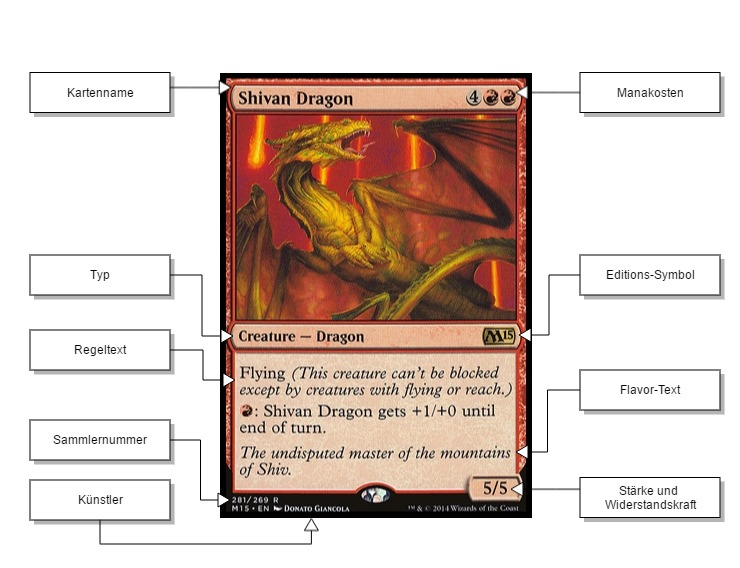
\includegraphics[width=\textwidth]{gfx/card.jpg}
	\caption{Bestandteile einer Karten}
	\label{fig:cardparts}
\end{figure}

\paragraph{Kartenname} 
Jede Karte hat einen eindeutigen Namen.

\paragraph{Typ}
Jede Karte hat einen bestimmten Typ. Außerdem kann eine Karte zusätzlich noch einen \emph{Subtyp/Untertyp} oder \emph{Supertyp} haben. Zum Beispiel: Der Shivan Dragon in \autoref{fig:cardparts} hat den Typ \emph{Kreatur} und als Untertyp \emph{Drache}. \cite{rulebook:2013}

\paragraph{Regeltext}
Enthält die \emph{Fähigkeiten} einer Karte, sofern vorhanden.

\paragraph{Flavor-Text}
Enthält Informationen über den Welt von \ac{MtG} und hat keinerlei Auswirkungen auf das Spielgeschehen.

\paragraph{Sammlernummer}
Hilft dabei die Karten einer Edition zu sortieren/organisieren.

\paragraph{Künstler}
Der Künstler von dem das Bild für die Karte stammt.

\paragraph{Stärke und Widerstandskraft}
Jede \emph{Kreatur} hat einen Wert für Stärke und Widerstandskraft. Die erste Zahl gibt die Stärke an und die zweite die Widerstandskraft.

\paragraph{Editions-Symbol}
Gibt Auskunft über die Edition aus der die Karte stammt. Die Farbe des Symbols verrät die Seltenheit: schwarz für häufige, silbern für nicht ganz so häufige, golden für seltene und rot-orange für sagenhafte Karten. \cite{rulebook:2013}

\paragraph{Manakosten}
Die Hauptressource in \ac{MtG} ist \emph{Mana}, welches von \emph{Ländern} produziert und für das spielen von \emph{Zaubern} benötigt wird. \cite{rulebook:2013}

\subsection{Kartentypen und Fähigkeiten}
Jede Karte in \ac{MtG} hat einen oder mehrere von den insgesamt sechs Typen \emph{(Land, Artefakt, Kreatur, Verzauberung, Planeswalker, Spontanzauber und Hexerei)}. An dem Kartentyp erkennt man wie sich die Karte verhält, das heißt wann man sie spielen kann und was danach mit ihr geschieht. \cite{rulebook:2013}

Viele Karten haben Texte, die sich auf das Spielgeschehen auswirken können, sogenannte Fähigkeiten. Aufgrund der großen Anzahl an Karten und der damit verbunden hohen Anzahl an verschiedenen Fähigkeiten werden diese in \emph{statische}, \emph{ausgelöste} und \emph{aktivierte Fähigkeiten} unterteilt. \cite{rulebook:2013}

\paragraph{Statische Fähigkeiten}
heißen so, da sie, solange sich die Karte im Spiel befindet, sich nicht verändern und konstant aktiv ist.

\paragraph{Ausgelöste Fähigkeiten}
sind Fähigkeiten, die durch ein bestimmtes Ereignis ausgelöst werden. Es gibt mehrere Formulierungen anhand derer man diese Art identifizieren kann. Die häufigsten sind \emph{wenn}, \emph{immer wenn} und \emph{zu}.

\paragraph{Aktivierte Fähigkeiten}
 erkennt man am Doppelpunkt. Sie werden in der Form \verb|[Kosten] : [Effekt]| angegeben, das heißt man muss etwas einsetzen, um die Fähigkeit zu aktivieren.

\paragraph{Schlüsselworte}
Fähigkeiten, die auf ein einzelnes Wort oder Satz gekürzt sind und eventuell einen Erinnerungstext haben, heißen \emph{Schlüsselwort-Fähigkeiten}. Meistens handelt es sich um \emph{statische Fähigkeiten}, aber \emph{ausgelöste} und \emph{aktivierte Fähigkeiten} sind auch möglich.


\section{Aufbau eines Decks}\label{ch:grundlagen:deck}
Ein Deck muss aus mindestens 60 Karten bestehen, wobei nach oben hin keine Grenzen gesetzt sind. Aus strategischer Sicht ist es aber sinnvoll möglichst nicht mehr als 60 Karten zu verwenden, da sonst die Wahrscheinlichkeit sinkt, die passende Karte zu ziehen. Des Weiteren ist es verboten mehr als vier Exemplare einer Karte im Deck zu haben, mit Ausnahme von Standardland-Karten, welche beliebig oft im Deck sein dürfen. Daraus ergeben sich folgende Richtlinien: \cite{rulebook:2013}
\begin{description}
    \item[Länder] Ein Deck sollte zwischen 35\% und 40\% aus Ländern bestehen
    \item[Kreaturen] Ein Deck sollte zwischen 25\% und 40\% aus Kreaturen bestehen. Dabei sollte beachtet werden, dass die Mana-Kosten gut verteilt sind
    \item[Sonstiges] Alles was nicht Land oder Kreatur ist und das Deck unterstützt
\end{description}

Turniere bieten eine Besonderheit, da es hier verschiedene Formate gibt. Bei manchen sind fast alle Karten erlaubt wohingegen bei anderen Formaten nur Karte der letzten paar Jahre erlaubt sind \cite{wotc:gameplay}.

\paragraph{Die Goldene Regel} Falls eine \ac{MtG} Karte dem Regelbuch widerspricht, hat die Karte Vorrang.  \cite{rulebook:2013}

\subsection{Deck-Typen}
Durch die große Menge an Karten und die goldene Regel ergeben sich viele verschiedene Spielweisen und Strategien nach denen man sein Deck ausrichten kann. Dadurch entstehen einige Decktypen, die die oben genannten Richtlinien für ihre Strategie anpassen. Decks die eine ähnliche Strategie haben oder gleich aufgebaut sind, werden unter einem Deck-Typ zusammengefasst \cite{haumagic}. Besonders starke Deck-Typen entstehen häufig durch die Analyse der einzelnen Karten und den Ergebnissen eines Decks in Turnieren \cite{haumagic}. Ein wichtiger Begriff ist hierbei die sogenannte Manakurve. Sie gibt an wie ausgewogen die Mana-Kosten in einem Deck sind - eine "hohe Manakurve" bedeutet, dass das Deck viele teurer Karten hat, wohingegen eine "niedrige Manakurve" bedeutet, dass viele günstige Karten enthalten sind. 

\paragraph{Aggro}
Bei der Aggro-Strategie geht es darum den Gegner möglichst früh mit den eigenen Kreaturen zu überrennen. Es wird durch die eigenen Kreaturen möglichst früh Druck auf den Gegener ausgeübt, um ihn so in die Verteidigung zu bringen. Entscheidend für die Strategie sind eine geringe Manakurve und viele kleine Kreaturen. \cite{wotc:gameplay}

\paragraph{Control}
Die Control-Strategie ist das genaue Gegenteil der Aggro-Strategie. Ziel ist es den Gegner solange in seiner Strategie zu stören, bis man im späten Spielverlauf die Partie mit eigenen wenigen starken Kreaturen das Spiel dominieren kann. Kontrolldecks setzten in erster Linie auf defensive Zauberkarten und wenige teure Kreaturen. \cite{wotc:gameplay}

\paragraph{Midrange}
Midrange-Decks sind eine Kombination aus Aggro- und Kontrolldecks. Sie sind sehr effizient und können sich an die Strategie des Gegners anpassen. Anstatt sich auf eine Strategie festzulegen wechseln Midrange-Decks je nach Situation zwischen aggressiver und defensiver Spielweise. \cite{wotc:gameplay}

\paragraph{Kombo}
Kombo-Decks nutzen Synergien die aus dem Zusammenspiel mehrerer Karten ergeben. Die Decks sind komplett darauf ausgerichtet, diese Synergien noch weiter zu unterstützen und dadurch die Oberhand in der Partie zu gewinnen. Aufgrund der Vielzahl an Karten gibt es unendlich viele Karten-Kombinationen. \cite{wotc:gameplay}


\section{Turniere}
Turniere werden ähnlich wie beim Schach nach dem Schweizer System gespielt. Dies ist eine Variante des Rundensystems bei der die Teilnehmer jede Runde spielen und die Paarungen sich anhand der bisherigen Spiel-Ergebnisse ergeben. Dadurch wird sichergestellt, dass Spieler mit ähnlichen Ergebnissen gegeneinander antreten \cite{starcitygames:swiss}. Wie in \autoref{tab:swisspairings} zu sehen, ist die Anzahl der gespielten Runden nach der Anzahl der Teilnehmer gestaffelt. 

Eine Runde wird nach dem \emph{Best-of-Three} Modus gespielt, das heißt die Runde ist beendet, sobald ein Spieler 2 Spiele gewonnen hat. 

\begin{table}[h] % t = top, also oben auf der Seite platzieren
    
    \caption{Anzahl der Runden die ab einer Teilnehmerzahl gespielt werden \cite{wotc:swiss}} 
    
    \myfloatalign
    \begin{tabular}{cc|cc}
        \toprule 
        Spieler & Runden & Spieler & Runden \\ 
        \midrule 
        2      & 1 & 129-212   & 8  \\ 
        3-4    & 2 & 213-384   & 9  \\ 
        5-8    & 3 & 385-672   & 10 \\ 
        9-16   & 4 & 673-1248  & 11 \\ 
        17-32  & 5 & 1249-2272 & 12 \\ 
        33-64  & 6 & 2273+     & 13 \\ 
        64-128 & 7 &           &  \\ 
        \bottomrule 
    \end{tabular}
    \label{tab:swisspairings}
\end{table}

\subsection{Match-Up}
Match-Up ist ein Begriff, welcher aus der Deckanalyse stammt und die Gewinn- und Verlustchancen eines Decks gegen ein anderes beschreibt. Der Wert wird oft in Prozentangaben wie 60:40 angegeben oder auch einfach nur als schlechtes oder gutes Match-Up.

\section{Graph-Datenbanken}
Ein Graph ist eine Sammlung von Objekten \emph{(Knoten)} und deren Verbindungen \emph{(Kanten)}. Graphen lassen sich vielfältig einsetzen, vom Straßennetz bis zur Krankengeschichte von Populationen \cite{robinsongraph:2015}. In \autoref{fig:simple_graph} sieht man eine einfache Unternehmenshierarchie als Graph dargestellt. 

\begin{figure}[h]
    \myfloatalign
    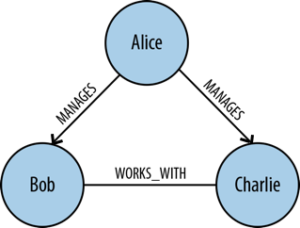
\includegraphics[width=0.65\textwidth]{gfx/simple_graph.png}
    \caption{Einfacher Graph \cite{neo4jblog:graph}}
    \label{fig:simple_graph}
\end{figure}

Ein \emph{Graph Datenbank Management System} (kurz \emph{Graph-Datenbank}) ist ein Datenbanken-Management-System, welches die \ac{CRUD} Eigenschaften unterstützt und ein Graph Daten-Modell bereitstellt \cite{robinsongraph:2015}.

Beziehungen in Graph-Datenbanken sind, im Gegensatz zu anderen Datenbank-Systemen, sogenannte \emph{first class citizens}. Dies bedeutet, dass Objekte mit einander verbunden werden können ohne dazu Fremdschlüssel oder ähnliche Konstrukte zu verwenden. Dadurch sind die Datenmodelle einfacher und ausdrucksvoller als Modelle von relationalen oder anderen \ac{NoSQL} Datenbanken. \cite{robinsongraph:2015} 

\subsection{Stärken von Graph-Datenbanken}
Aufgrund der Tatsache, dass Abfragen nur auf einem Teil des Graphen arbeiten, bleibt die Performance einer Graph-Datenbank relativ konstant auch wenn der Datensatz wächst. Bei relationalen Datenbank Abfragen mit vielen joins hingegen verschlechtert sich die Abfrageperformance bei zunehmenden Datensatz. \cite{robinsongraph:2015}

Eine weitere Stärke von Graph-Datenbanken ist ihr flexibles Datenmodell. Es können neue Beziehungen, Knoten oder Untergraphen zu bestehenden Strukturen hinzugefügt werden ohne, dass es dabei zu Konflikten mit vorhandene Abfragen kommt. Dies bedeutet, dass das Datenmodell nicht ausführlich mit allen Details vor Projektbeginn vorhanden sein muss, sondern an geänderte Anforderungen im laufe des Projekts angepasst werden kann. \cite{robinsongraph:2015}

% !TEX root = ../TUCthesis.tex
%****************************************************
\chapter{Methode}\label{ch:methode}
%****************************************************

% !TEX root = ../TUCthesis.tex
%****************************************************
\section{Analyse der Anforderungen}\label{ch:analyse}
%****************************************************

\subsection{Kartensuche}
%- Karte:
%    Suche nach verschiedenen Attributen oft auch kombiniert. zb
%         nur Künstler X 
%         alle Karten vom Typ X die in Edition Y und Farbe Z haben
%    -> Verknüfung der verschiedenen Attribute = Relationship/Beziehungen
%    -> Echtzeit (Web): dh. unter 150ms
%    
Aufgrund der großen Anzahl an Karten \emph{(>15.000 \cite{mtgjson})} ist eine Suchfunktion hervorragend geeignet, um bestimmte oder ähnliche Karten zu finden. Wie in \ref{ch:grundlagen:aufbau} beschrieben, enthält eine Karte viele verschiedenen Attribute. Daher ist es sinnvoll bei einer Suchfunktion die \emph{Verknüpfung dieser Attribute} zu erlauben, sodass zum Beispiel nach allen Karten eines Künstlers, die in einem bestimmten Set erschienen sind, gesucht werden kann. 

Da eine solche Suchfunktion oftmals webbasiert ist, muss es möglich sein, dass ein Benutzer die Ergebnisse in Echtzeit erhält.



\subsection{Deckbau}
%- Deck Analyse:
%    * Berechnung von Kostenverteilung => Manakurve => Erklären warum Analyse (Anzahl Kreaturen, Manakurve etc.) von Decks hilfreich beim Deckbau
%    * Aufzählung von Karten-typen / Farben
%    -> Verknüfung von Deck mit Karten-Daten
%    -> Echtzeit (Web): dh. unter 150ms
% 
Wie in \ref{ch:grundlagen:deck} zu sehen ist, gibt es verschiedene Richtlinien die beim Deckbau zu beachten sind, sofern man ein gutes Deck erstellen möchte. Diese Richtlinien können sich jedoch abhängig vom Deck-Typen stark unterscheiden. Ein hilfreiches Werkzeug beim Deckbau ist daher die Deck-Analyse.

Die Berechnung der Kostenverteilung, das heißt die Manakurve, hilft ... %TODO
Auch die Verteilung der einzelnen Kartentypen, das heißt die Anzahl der Kreaturen, Zauber, usw., ist für verschiedene Deck-Typen wichtig. So ist für ein Aggro-Deck eine hohe Anzahl an Kreaturen wichtig, wohingegen ein Control-Deck eher eine hohe Anzahl an Zaubern enthält. Da sich viele Decks aber nicht nur auf eine Farbe beschränken, ist es auch wichtig zu wissen, wie die Farben im Deck verteilt sind, um so die Manaquellen im Deck entsprechend zu verteilen. 

Beim Deckbau werden in der Regel nur die Anzahl der Karte im Deck und ihr Name angegeben. Aus diesem Grund ist es wichtig den Inhalt des Decks mit den Karten-Daten zu verknüpfen, um Zugriff auf die benötigten Attribute zu haben. Außerdem sollte auch hier die Analyse die Ergebnisse in Echtzeit liefern, damit sich die Funktion für webbasierte Anwendungen eignet.

\subsection{Turniere}
%- Turnier Analyse:
%    * Matchup für Deck-Typ X
%    * Erfolgreichster Spieler / Deck
%    -> Verknüpfung von Decks mit Turnier-Matches und Spielern
%    -> Echtzeit (Web): dh. unter 150ms
Sowohl für professionelle Turnierspieler als auch für Amateure ist die Analyse vergangener Turniere wichtig, um ihre Decks bestmöglich an potentiell überlegende Decks anzupassen. Dazu ist die Berechnung des Match-Ups für ein Deck-Typ wichtig. Dazu müssen die einzelnen Ergebnisse einer Runde eines Turniers mit den Decks verknüpft werden.

Ein weitere interessante Information ist die des erfolgreichsten Spielers oder des erfolgreichsten Deck(-Typen) über eine Auswahl an Turnieren. 

Wie in den vorherigen Fällen ist auch hier eine webbasierte Anwendung wünschenswert und damit die Berechnung der Resultate in Echtzeit.


% !TEX root = ../TUCthesis.tex
%****************************************************
\section{Potentielle Ansätze und Probleme}\label{ch:ansaetze-probleme}
%****************************************************

\subsection{Relationale Datenbanken}
%* Ansatz: RDBMS da etabliert -> gut für suche
% https://books.google.nl/books?id=RTvcCQAAQBAJ&pg=PA1&num=10&hl=de&source=gbs_toc_r&cad=3#v=onepage&q&f=true
%* Beispiel: komplexe SQL Abfrage *(siehe expose)*
%* Komplizierte Abfragen / viele JOINs *(Bezug zu Aufbau Karte)*
% Skalierbarkeit?

Ein Ansatz, welcher sich für kleine Online-Shops eignet, ist die Karten-Daten in einer relationalen Datenbank zu speichern \cite{johnson2013online}. Da ein Online-Shop nur einen Teil der Attribute einer Karte, wie Name, Seltenheit und Set, benötigt, kann das Datenbank Schema aus ein bis zwei Tabellen bestehen, die diese Informationen speichern. Für eine komplexe Suchfunktion, die alle Attribute einer Karte berücksichtigt, eignet sich dieser Ansatz allerdings nicht, da hier viele Tabellen benötigt werden, um die Daten zu speichern. Bei Daten mit vielen Beziehungen untereinander sorgen Relationale Datenbanken für komplexe Abfragen mit vielen JOINS, da diese hoch-strukturierte Daten nicht unterstützen \cite{robinsongraph:2015}. In \autoref{listing:complex.sql} ist beispielhaft eine komplexe Suchanfrage mit 7 benötigten JOINS angegeben.

\begin{listing}[H]
    \caption{Komplexe SQL-Abfrage}
    \label{listing:complex.sql}
    \begin{lstlisting}[language=SQL]
SELECT * FROM `translations` AS `t` 
JOIN `cards` ON `cards`.`id` = `t`.`card_id`
JOIN `cards_in_set` ON `cards_in_set`.`card_id` = `t`.`card_id`
JOIN `types` ON `cards`.`type_id` = `types`.`id`
JOIN `card_colors` ON `cards`.`id` = `card_colors`.`card_id`
JOIN `card_has_ability` ON `cards`.`id` = `card_has_ability`.`card_id`
JOIN `keyword_abilities` ON `card_has_ability`.`ability_id` = `keyword_abilities`.`id`
JOIN `sets` ON `sets`.`id` = `cards_in_set`.`set_id`
WHERE
    `sets`.release > "2001-01-01" AND
    `cards_in_set`.`rarity` = "RARE" AND
    `t`.`lang` = "German" AND
    `card_colors`.color = "BLUE" AND
    `types`.`type` = "Creature" AND
    `keyword_abilities`.`name` = "Flying" AND
    `cards`.`cmc` <= 5
    \end{lstlisting}
\end{listing}


\subsection{NoSQL Datenbanken}
% https://books.google.nl/books?id=RTvcCQAAQBAJ&pg=PA1&num=10&hl=de&source=gbs_toc_r&cad=3#v=onepage&q&f=true
% S.15 ,S.18-19
\ac{NoSQL} Datenbanken wie Key-Value-, Document- oder Column-oriented Stores eignen sich nicht für Daten mit vielen Verknüpfungen, da sie die Daten nicht verbunden speichern. Eine Ausnahme sind die Graph-Datenbanken, da sie die Daten als Graph speichern, unterstützen sie daher Daten mit vielen Beziehungen untereinander von vornherein. \cite{robinsongraph:2015}

% TODO
\cite{jaiswal2013comparative}
\cite{vicknair2010comparison}




% !TEX root = ../TUCthesis.tex
%****************************************************
\section{Software-Design}\label{ch:design}
%****************************************************

\subsection{Daten-Schemata}
%%%%%%%%%%%%%%%%%%%%%%%%%%%%%%%%%%%%%%%
% Schemata für DB
%   * Relational
%   * Graph: evtl. verschiede Anätze für Model
%%%%%%%%%%%%%%%%%%%%%%%%%%%%%%%%%%%%%%%
Um das Daten-Schema für die relationale Datenbank darzustellen, wird \ac{UML} verwendet. Die Vorteile von \ac{UML} liegen im Gegensatz zum \ac{ER-Modell} darin, dass es weit verbreitet, standardisiert ist und sich gut für \ac{OOP} eignet \cite{teorey2011database}. In \autoref{fig:uml:schema} befindet sich das Daten-Schema für die relationale Datenbank.

Wie viele Graph-Datenbanken nutzt auch Neo4j das Property-Graph-Modell um Daten darzustellen. Dieses Modell ist ein Untertyp des mathematischen Graph-Modells. Property-Graph-Modelle sind einfacher, aussagekräftiger und geben Beziehungen explizit an. \ac{RDBMS} verwenden Fremdschlüssel, um Beziehungen implizit anzugeben \cite{lal2015neo4j}. In \autoref{fig:graph:schema} befindet sich ein möglicher Ansatz für ein Schema.

\begin{figure}[H]
    \myfloatalign
    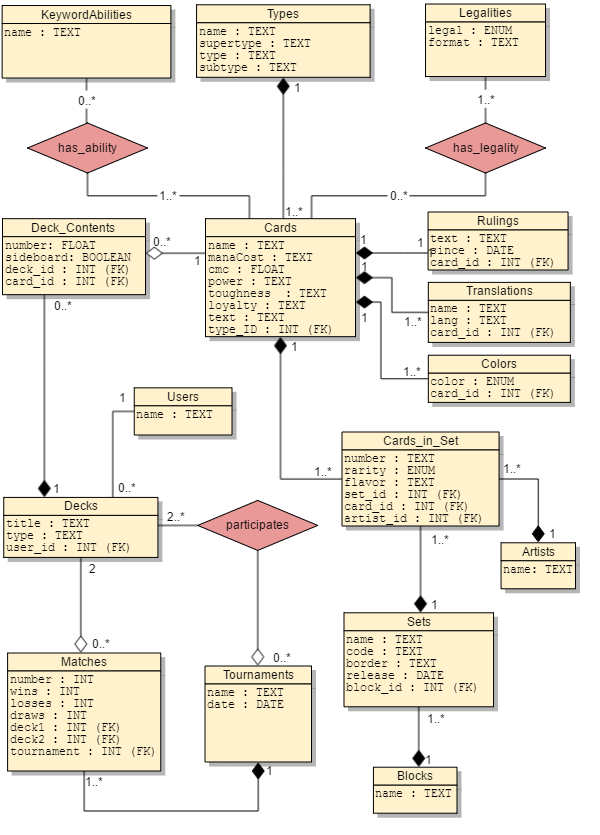
\includegraphics[width=\textwidth]{gfx/erm.png}
    \caption{Schema für relationale Datenbank}
    \label{fig:uml:schema}
\end{figure}

\begin{figure}[H]
    \myfloatalign
    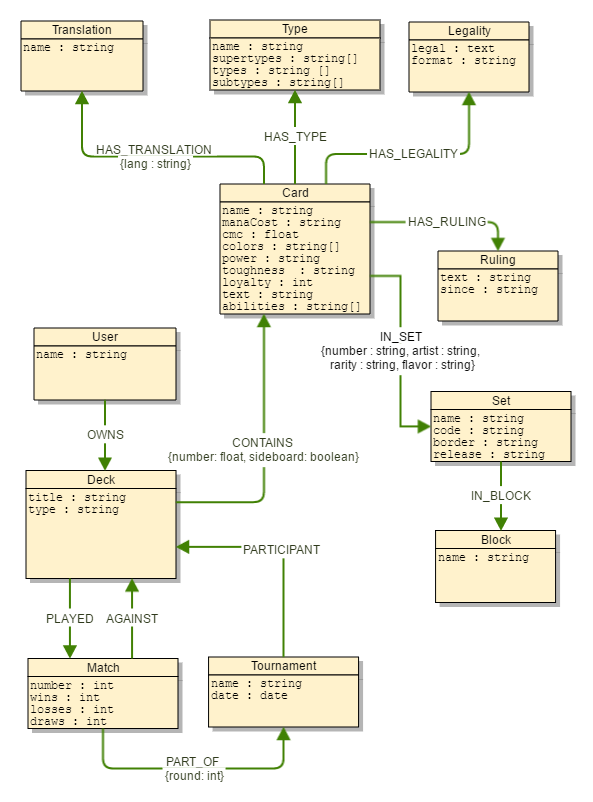
\includegraphics[width=\textwidth]{gfx/graph.png}
    \caption{Schema für Graph-Datenbank}
    \label{fig:graph:schema}
\end{figure}

\subsection{Beschreibung der Software-Komponenten}
%%%%%%%%%%%%%%%%%%%%%%%%%%%%%%%%%%%%%%%
%  * Dekomposition -> Softwarekomponenten + Beschreibung der Schnittstellen (Komponenten-Diagramm, siehe "SW-Architektur Webserver")
%  * Schnittstellenbeschreibung -> API für jedes Modul Model + Tabelle + Description (Klassen-Diagramm)
%%%%%%%%%%%%%%%%%%%%%%%%%%%%%%%%%%%%%%%

\begin{figure}[H]
    \myfloatalign
    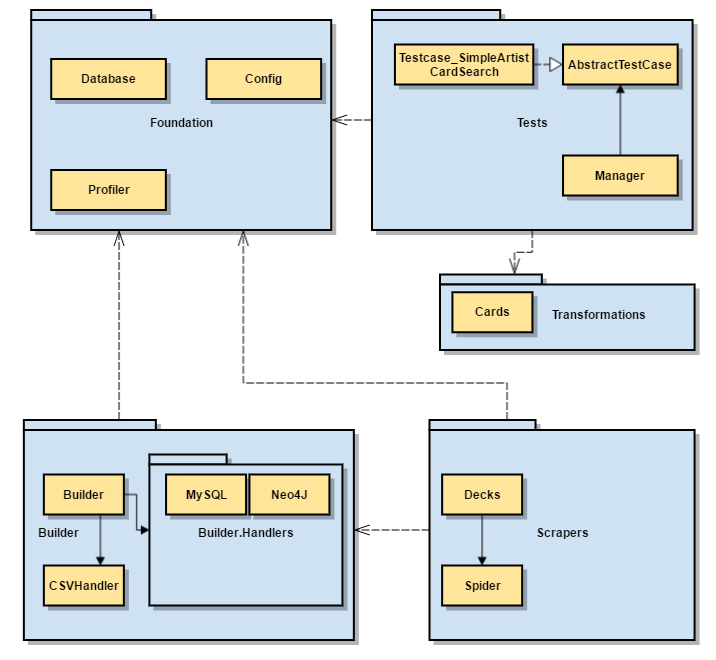
\includegraphics[width=\textwidth]{gfx/sw-components.png}
    \caption{Software-Komponenten}
    \label{fig:sw-components}
\end{figure}
\begin{description}
    \item[Builder] \hfill \\
        Das Package Builder ist zuständig für das erstellen und befüllen der Datenbanken.
    
    \item[Builder.Handlers]  \hfill \\
        Das Package Builder.Handlers enthält die Implementierungen für die konkreten Datenbanken
    
    \item[Scrapers]  \hfill \\
         Das Package Scrapers lädt Decks von mtgtop8 \footnote{mtgtop8 - http://mtgtop8.com/} herunter, um einen Datensatz für Decks und Turniere zu erstellen
    
    \item[Tests]  \hfill \\
        Enthält die konkreten Testfälle
    
    \item[Transformers]  \hfill \\
        Das Package Transformers ist zuständig für das Transformieren von Daten in eine vorgegebene Datenstruktur.
\end{description}

\subsection{Beschreibung der Schnittstellen}
%%% Beschreibung der Packet Schnittstellen. Scraper.Decks nutzt Spider um ..., Scraper.Decks nutzt Config? um ..
%%% evtl als liste ala:
%%% Scraper.Decks nutzt die folgenden Schnittstellen:
%%%   * Spider: Wird genutzt um webpage inhalt zu erhalten
%%%   * Foundation.Config: wird genutzt um xy zu erhalten
%%%   * ...
\subsubsection*{Builder}
Die Komponente \verb|Builder| nutzt die folgenden Schnittstellen:
\begin{description}
    \item[Foundation] wird genutzt um ein Datenbank-Verbindungen zu erstellen
\end{description}

\subsubsection*{Scrapers}
Die Komponente \verb|Scrapers| nutzt die folgenden Schnittstellen:
\begin{description}
    \item[Foundation] wird genutzt um auf die Konfiguration zuzugreifen
    
    \item[Builder] wird genutzt um die Decks in \ac{CSV} Dateien zu speichern
\end{description}

\subsubsection*{Tests}
Die Komponente \verb|Tests| nutzt die folgenden Schnittstellen:
\begin{description}
    \item[Foundation] wird genutzt um ein Datenbank-Verbindungen zu erstellen und mit dem \verb|Profiler| die Testfälle zu überwachen
    
    \item[Transformations] um die ausgelesenen Daten in eine passende Datenstruktur zu überführen
\end{description}

% !TEX root = ../TUCthesis.tex
%****************************************************
\section{Implementierung}\label{ch:implementierung}
%****************************************************

% Schnittstellenrealisierung -> Interaktionsdiagramm

\subsection{Klassendiagramme}
%%%%%%%%%%%
%% Tests %%
%%%%%%%%%%%
\subsubsection{Tests.AbstractTestCase}
Die Abstrakte Klasse \verb|Tests.AbstractTestCase| hat die folgenden Schnittstellen:

\begin{figure}[H]
    \myfloatalign
    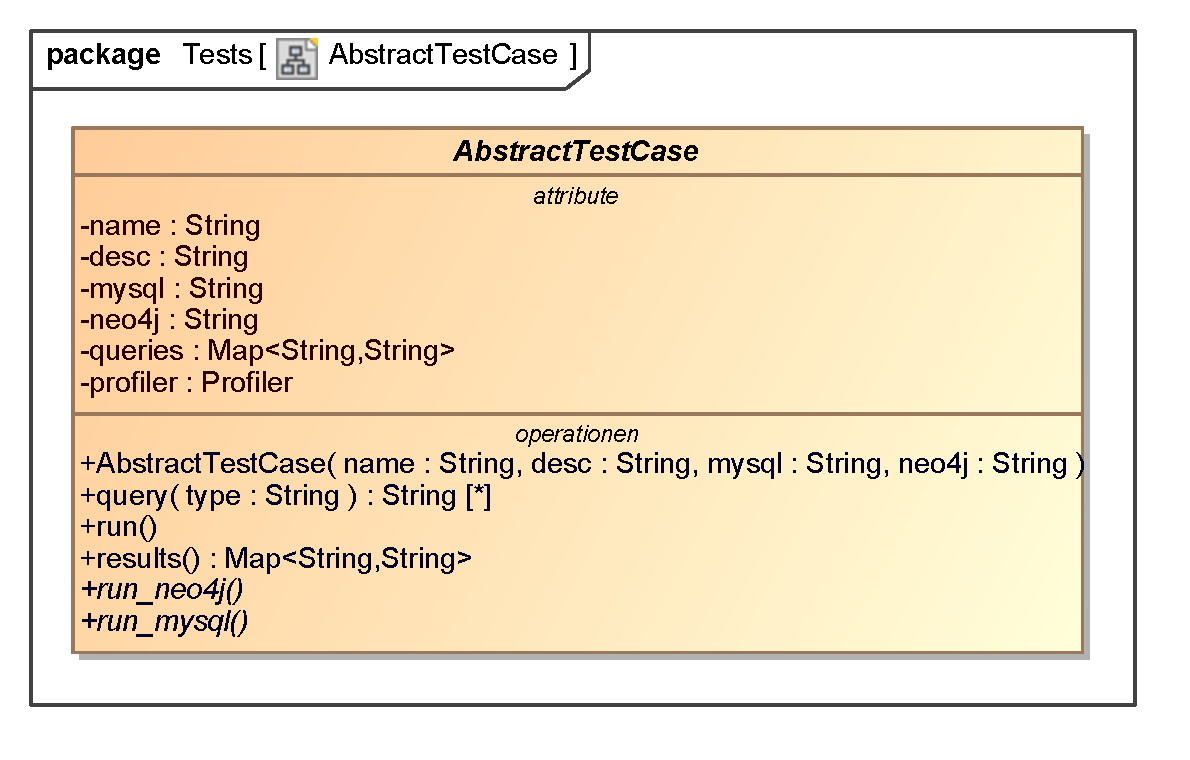
\includegraphics[width=0.85\textwidth]{gfx/MtGDeepAnalysis/AbstractTestCase.eps}
    \caption{Klassendiagramm Tests.AbstractTestCase}
    \label{fig:class:tests.abstracttestcase}
\end{figure}

\begin{description}
    \item[constructor(name, desc, mysql, neo4j)] \hfill \\
    Setzt den Namen \verb|name| und die Beschreibung \verb|desc| des Testfalls. Außerdem werden die Schlüssel \verb|mysql| und \verb|neo4j| festgelegt, welche für die Testergebnisse benutzt werden. Die Liste der Argumente befindet sich in \autoref{tab:tests.abstracttestcase.constructor}
    
    \item[query(type)] \hfill \\
    Gibt alle Abfragen für \verb|type = [mysql, neo4j]| die in dem Test ausgeführt werden zurück.
    
    \item[run()] \hfill \\
    Führt Test durch.
    
    \item[results()] \hfill \\
    Gibt aufgezeichnete Ergebnisse zurück nachdem der Test ausgeführt wurde.
    
    \item[run\_neo4j()] \hfill \\
    Testfall für Neo4j-Datenbank.
    
    \item[run\_mysql()] \hfill \\
    Testfall für MySQL-Datenbank.
\end{description}


\begin{table}[h]
    \caption{Tests.AbstractTestCase::constructor(name : string, desc : string, mysql : string, neo4j : string)} 
    \myfloatalign
    \begin{tabularx}{\textwidth}{lX}
        \toprule 
        \tableheadline{Eingabe} & \tableheadline{Beschreibung} \\ 
        \midrule 
        \verb|name : string| & Name des Testfalls \\
        \verb|desc : string| & Beschreibung des Testfalls \\
        \verb|mysql : string| & Schlüssel für MySQL-Testergebnisse \\
        \verb|neo4j : string| & Schlüssel für Neo4j-Testergebnisse \\
        \bottomrule 
    \end{tabularx}
    \label{tab:tests.abstracttestcase.constructor}
\end{table}

\subsubsection{Tests.CardTestcase}
Die Abstrakte Klasse \verb|Tests.CardTestcase| hat die folgenden Schnittstellen:

\begin{figure}[H]
    \myfloatalign
    \includegraphics[width=0.65\textwidth]{gfx/MtGDeepAnalysis/CardTestcase.eps}
    \caption{Klassendiagramm Tests.CardTestcase}
    \label{fig:class:tests.CardTestcase}
\end{figure}

\begin{description}
    \item[init\_queries()] \hfill \\
    Fügt Standardabfragen zu \verb|queries| hinzu, welche für die Kartentests gebraucht werden
        
    \item[run\_neo4j()] \hfill \\
    Cypher-Abfragen ausführen und Karten in Datenstruktur \verb|Transformations.Cards| überführen
    
    \item[run\_mysql()] \hfill \\
    SQL-Abfragen ausführen und Karten in Datenstruktur \verb|Transformations.Cards| überführen
\end{description}

\subsubsection{Tests.Manager}
Die Klasse \verb|Tests.Manager| hat die folgenden Schnittstellen:

\begin{figure}[H]
    \myfloatalign
    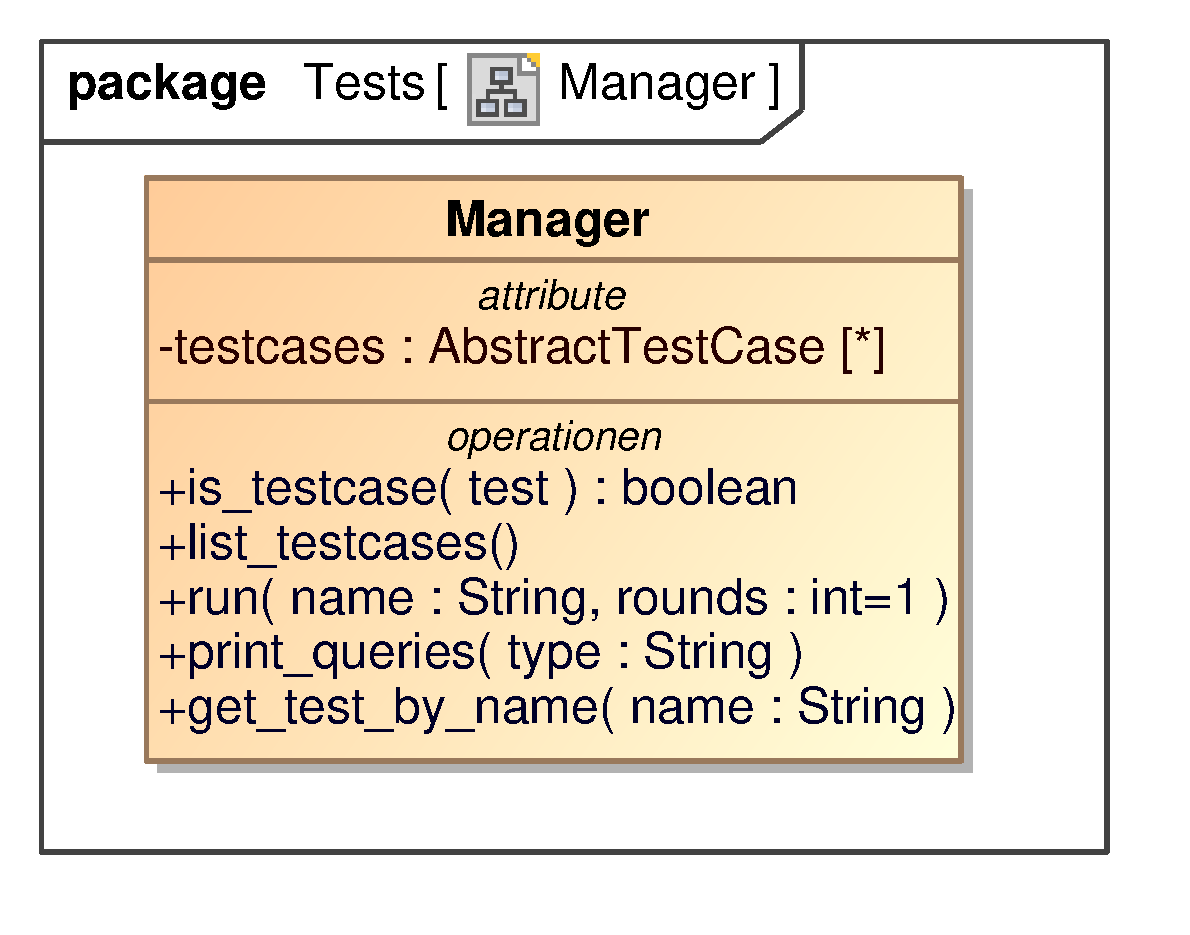
\includegraphics[width=0.65\textwidth]{gfx/MtGDeepAnalysis/Manager.eps}
    \caption{Klassendiagramm Tests.Manager}
    \label{fig:class:tests.manager}
\end{figure}

\begin{description}
    \item[Manager()] \hfill \\
    Lädt alle Testfälle und speichert diese in \verb|testcases|
    
    \item[is\_testcase(test)] \hfill \\
    Prüft ob ein Objekt \verb|test| ein Testfall ist, das heißt von \verb|Tests.AbstractTestCase| abgeleitet ist.
    
    \item[list\_testcases()] \hfill \\
    Gibt eine Liste der verfügbaren Tests in \verb|testcases| aus
    
    \item[run(name, rounds)] \hfill \\
    Führt den Testfall \verb|name| \verb|rounds|-mal hintereinander aus
    
    \item[print\_queries(name)] \hfill \\
    Gibt alle Abfragen des Testfalls \verb|name| aus.
    
    \item[get\_test\_by\_name(name)] \hfill \\
    Gibt den Testfall \verb|name| zurück, sofern dieser sich in \verb|testcases| befindet
\end{description}

\subsubsection{Tests.Testcase\_ComplexCardSearch}
Die Klasse \verb|Tests.Testcase_ComplexCardSearch| hat die folgenden Schnittstellen:

\begin{figure}[H]
    \myfloatalign
    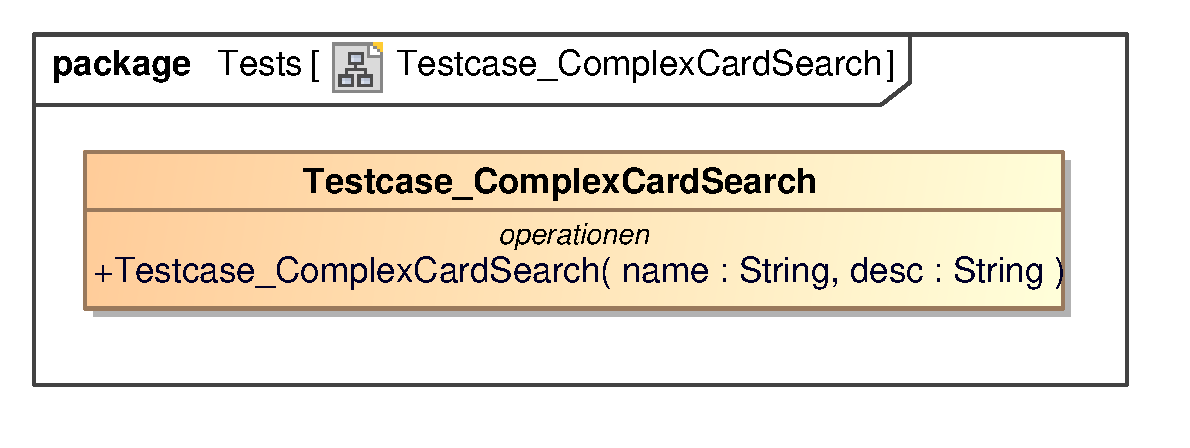
\includegraphics[width=0.75\textwidth]{gfx/MtGDeepAnalysis/Testcase_ComplexCardSearch.eps}
    \caption{Klassendiagramm Tests.Testcase\_ComplexCardSearch}
    \label{fig:class:tests.Testcase_ComplexCardSearch}
\end{figure}

\begin{description}
    \item[Testcase\_ComplexCardSearch(name, desc)] \hfill \\
    Fügt Abfragen des Testfalls zu \verb|queries| hinzu
\end{description}

\subsubsection{Tests.Testcase\_Matchup}
Die Klasse \verb|Tests.Testcase_Matchup| hat die folgenden Schnittstellen:

\begin{figure}[H]
    \myfloatalign
    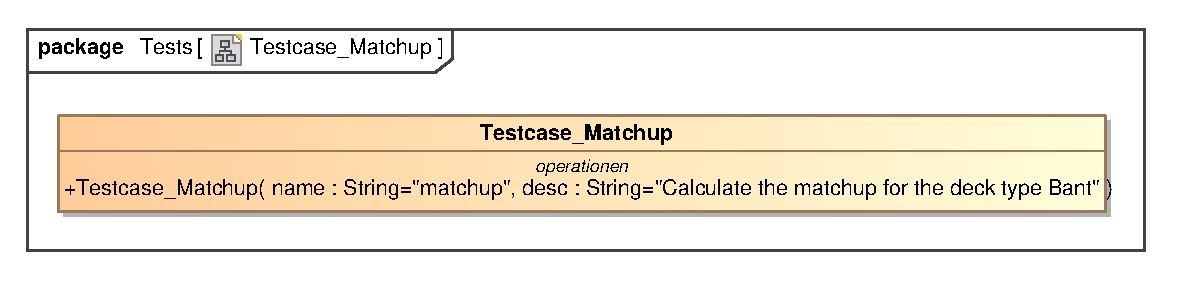
\includegraphics[width=0.75\textwidth]{gfx/MtGDeepAnalysis/Testcase_Matchup.eps}
    \caption{Klassendiagramm Tests.Testcase\_Matchup}
    \label{fig:class:tests.Testcase_Matchup}
\end{figure}

\begin{description}
    \item[Testcase\_Matchup(name, desc)] \hfill \\
    Fügt Abfragen des Testfalls zu \verb|queries| hinzu
\end{description}

\subsubsection{Tests.Testcase\_SimpleArtistCardSearch}
Die Klasse \verb|Tests.Testcase_SimpleArtistCardSearch| hat die folgenden Schnittstellen:

\begin{figure}[H]
    \myfloatalign
    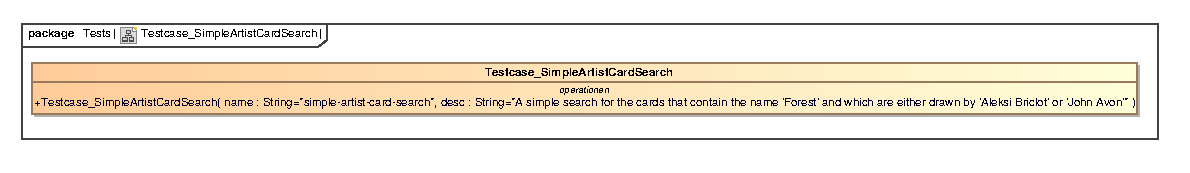
\includegraphics[width=0.75\textwidth]{gfx/MtGDeepAnalysis/Testcase_SimpleArtistCardSearch.eps}
    \caption{Klassendiagramm Tests.Testcase\_SimpleArtistCardSearch}
    \label{fig:class:tests.Testcase_SimpleArtistCardSearch}
\end{figure}

\begin{description}
    \item[Testcase\_SimpleArtistCardSearch(name, desc)] \hfill \\
    Fügt Abfragen des Testfalls zu \verb|queries| hinzu
\end{description}

\subsubsection{Tests.Testcase\_SimpleKeywordAbilitySearch}
Die Klasse \verb|Tests.Testcase_SimpleKeywordAbilitySearch| hat die folgenden Schnittstellen:

\begin{figure}[H]
    \myfloatalign
    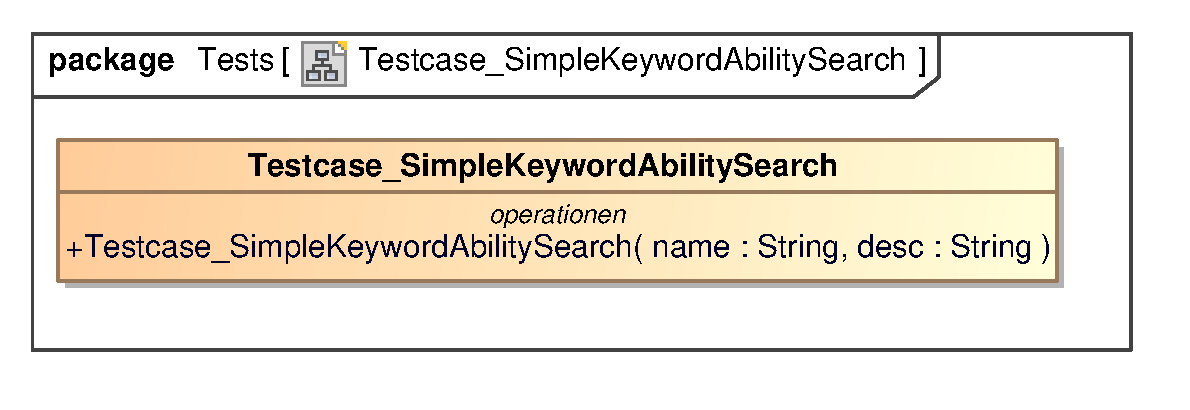
\includegraphics[width=0.75\textwidth]{gfx/MtGDeepAnalysis/Testcase_SimpleKeywordAbilitySearch.eps}
    \caption{Klassendiagramm Tests.Testcase\_SimpleKeywordAbilitySearch}
    \label{fig:class:tests.Testcase_SimpleKeywordAbilitySearch}
\end{figure}

\begin{description}
    \item[Testcase\_SimpleKeywordAbilitySearch(name, desc)] \hfill \\
    Fügt Abfragen des Testfalls zu \verb|queries| hinzu
\end{description}

\subsubsection{Tests.Testcase\_TopTenDecks}
Die Klasse \verb|Tests.Testcase_TopTenDecks| hat die folgenden Schnittstellen:

\begin{figure}[H]
    \myfloatalign
    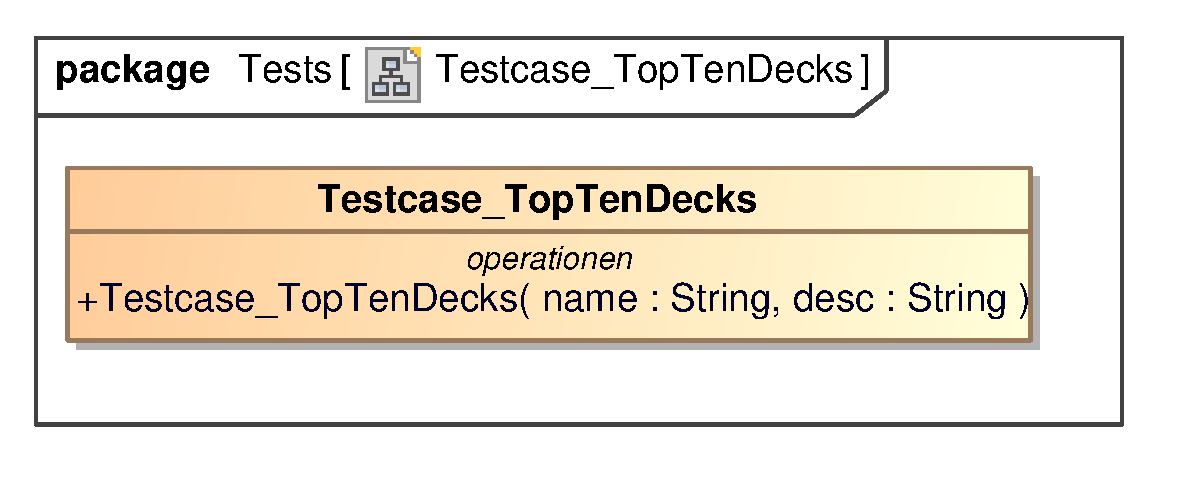
\includegraphics[width=0.75\textwidth]{gfx/MtGDeepAnalysis/Testcase_TopTenDecks.eps}
    \caption{Klassendiagramm Tests.Testcase\_TopTenDecks}
    \label{fig:class:tests.Testcase_TopTenDecks}
\end{figure}

\begin{description}
    \item[Testcase\_TopTenDecks(name, desc)] \hfill \\
    Fügt Abfragen des Testfalls zu \verb|queries| hinzu
\end{description}

%%%%%%%%%%%%%%%%
%% Foundation %%
%%%%%%%%%%%%%%%%
\subsubsection{Foundation.Config}
Die Klasse \verb|Foundation.Config| hat die folgenden Schnittstellen:

\begin{figure}[H]
    \myfloatalign
    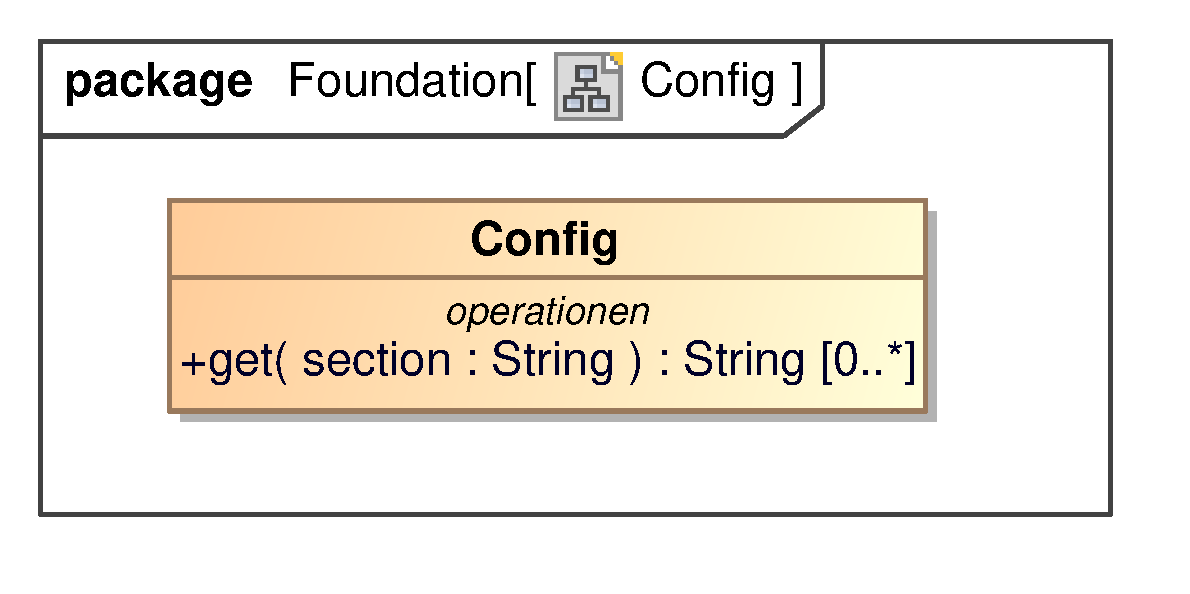
\includegraphics[width=0.75\textwidth]{gfx/MtGDeepAnalysis/Config.eps}
    \caption{Klassendiagramm Foundation.Config}
    \label{fig:class:foundation.config}
\end{figure}

\begin{description}
    \item[Config()] \hfill \\
    Lädt die Konfigurationsdatei Datei \verb|config.ini|
    
    \item[get(section)] \hfill \\
    Gibt einen Konfigurationsabschnitt \verb|section| als \verb|string[]| aus der Datei \verb|config.ini| zurück
\end{description}


\subsubsection{Foundation.Database}
Die Klasse \verb|Foundation.Database| hat die folgenden Schnittstellen:

\begin{figure}[H]
    \myfloatalign
    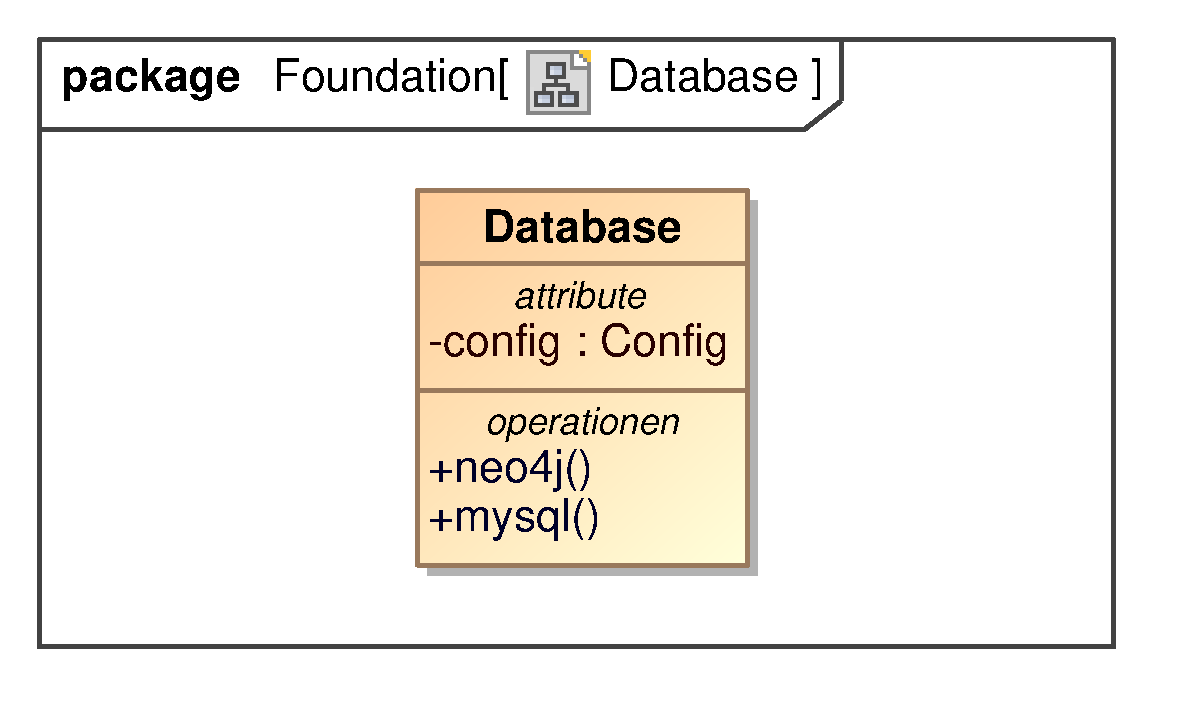
\includegraphics[width=0.75\textwidth]{gfx/MtGDeepAnalysis/Database.eps}
    \caption{Klassendiagramm Foundation.Database}
    \label{fig:class:foundation.database}
\end{figure}

\begin{description}
    \item[Database()] \hfill \\
    Erstellt eine neue \verb|Foundation.Config| Instanz und speichert diese in \verb|config|.
    
    \item[neo4j()] \hfill \\
    Gibt eine neue Neo4j Datenbank-Instanz zurück.
    
    \item[mysql()] \hfill \\
    Gibt eine neue Mysql Datenbank-Instanz zurück.
\end{description}

\subsubsection{Foundation.Profiler}
Die Klasse \verb|Foundation.Profiler| hat die folgenden Schnittstellen:

\begin{figure}[H]
    \myfloatalign
    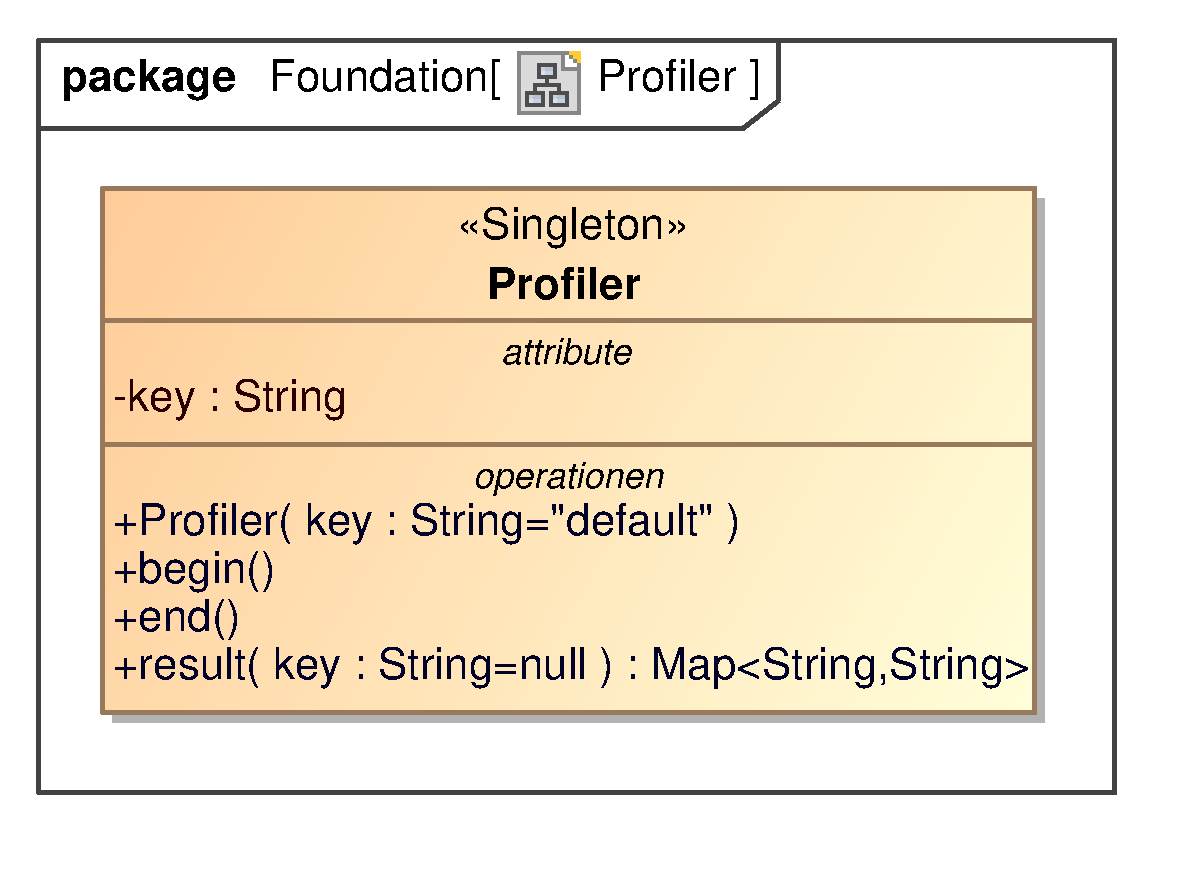
\includegraphics[width=0.75\textwidth]{gfx/MtGDeepAnalysis/Profiler.eps}
    \caption{Klassendiagramm Foundation.Profiler}
    \label{fig:class:foundation.profiler}
\end{figure}

\begin{description}
    \item[Profiler(key)] \hfill \\
    Erstellt eine neue \verb|Profiler| Instanz mit dem Schlüssel \verb|key| falls noch keine Vorhanden ist
    
    \item[begin()] \hfill \\
    Startet den Profiler
    
    \item[end()] \hfill \\
    Beendet der Profiler und speichert die gemessene Laufzeit und Speicherverbrauch
    
    \item[result(key : String)] \hfill \\
    Gibt das Ergebnis für des Profilers \verb|key| zurück
\end{description}

%%%%%%%%%%%%%%
%% Scrapers %%
%%%%%%%%%%%%%%
\subsubsection{Scrapers.Spider}
Die Klasse \verb|Scrapers.Spider| hat die folgenden Schnittstellen:

\begin{figure}[H]
    \myfloatalign
    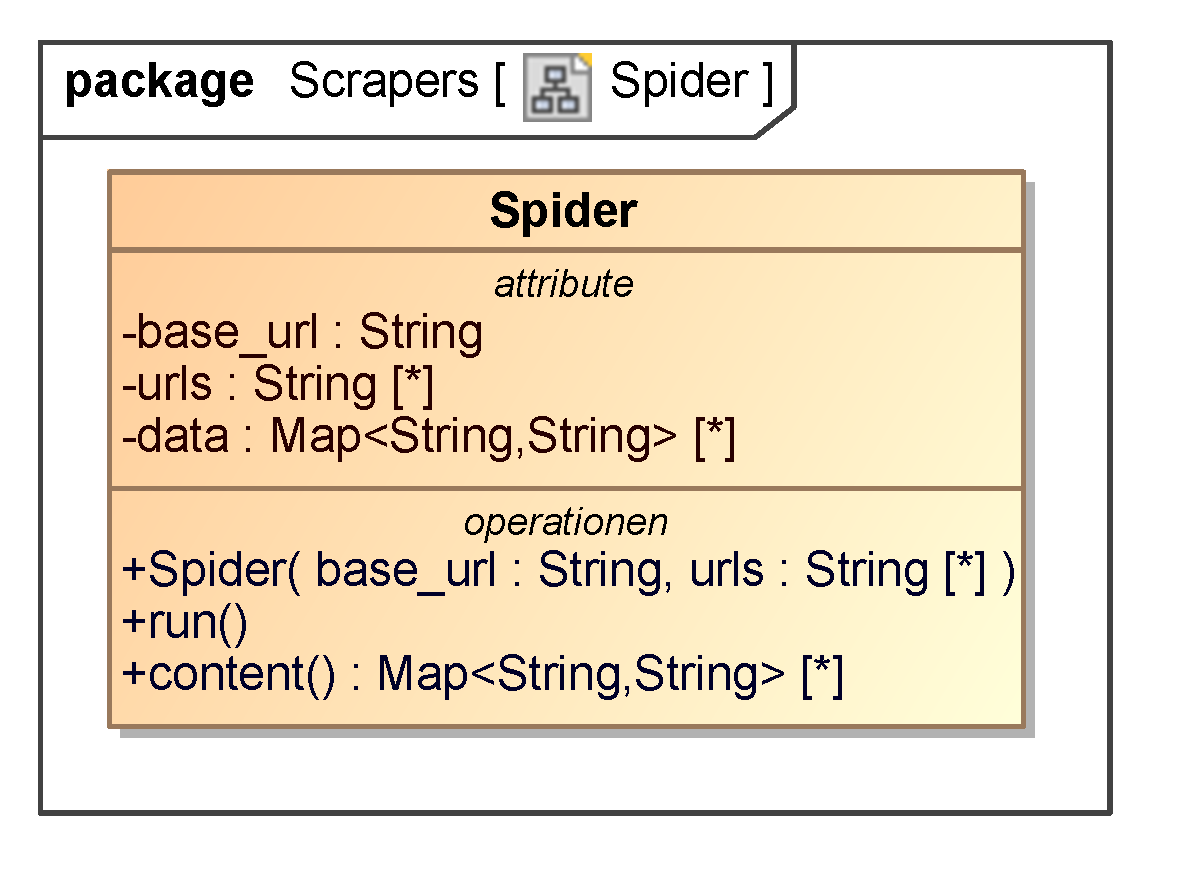
\includegraphics[width=0.65\textwidth]{gfx/MtGDeepAnalysis/Spider.eps}
    \caption{Klassendiagramm Scrapers.Spider}
    \label{fig:class:Scrapers.Spider}
\end{figure}

\begin{description}
    \item[Spider(base\_url, urls)] \hfill \\
    Initiert die Spider Klasse
    
    \item[run] \hfill \\
    Lädt die Decks von \verb|urls| und speichert diese
    
    \item[content()] \hfill \\
    Gibt die heruntergeladenen Decks zurück
\end{description}

\subsubsection{Scrapers.Decks}
Die Klasse \verb|Scrapers.Decks| hat die folgenden Schnittstellen:

\begin{figure}[H]
    \myfloatalign
    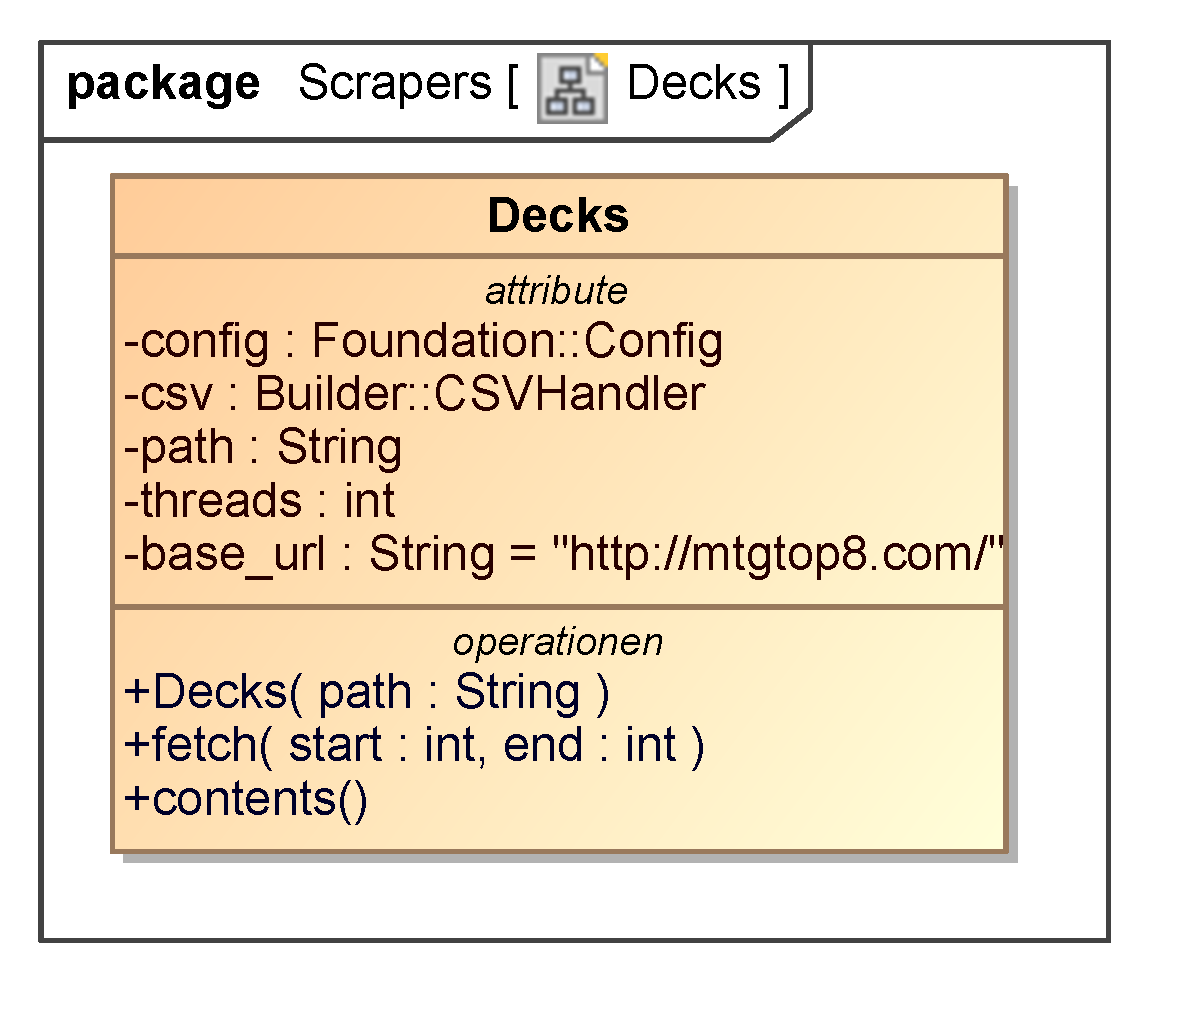
\includegraphics[width=0.65\textwidth]{gfx/MtGDeepAnalysis/Decks.eps}
    \caption{Klassendiagramm Scrapers.Decks}
    \label{fig:class:Scrapers.Decks}
\end{figure}

\begin{description}
    \item[Decks(path)] \hfill \\
    Initiert den CSVHandler mit \verb|path|
    
    \item[fetch(start, end)] \hfill \\
    Lädt die Decks per \verb|Spider| und speichert diese per \verb|CSVHandler| in einer \verb|decks.csv|
    
    \item[contents()] \hfill \\
    Extrahiert die Karten aus den heruntergeladenen Decks und speichert diese in eigener \ac{CSV} Datei
\end{description}

%%%%%%%%%%%%%%%%%%%%%
%% Transformations %%
%%%%%%%%%%%%%%%%%%%%%
\subsubsection{Transformations.Cards}
Die Klasse \verb|Transformations.Cards| hat die folgenden Schnittstellen:

\begin{figure}[H]
    \myfloatalign
    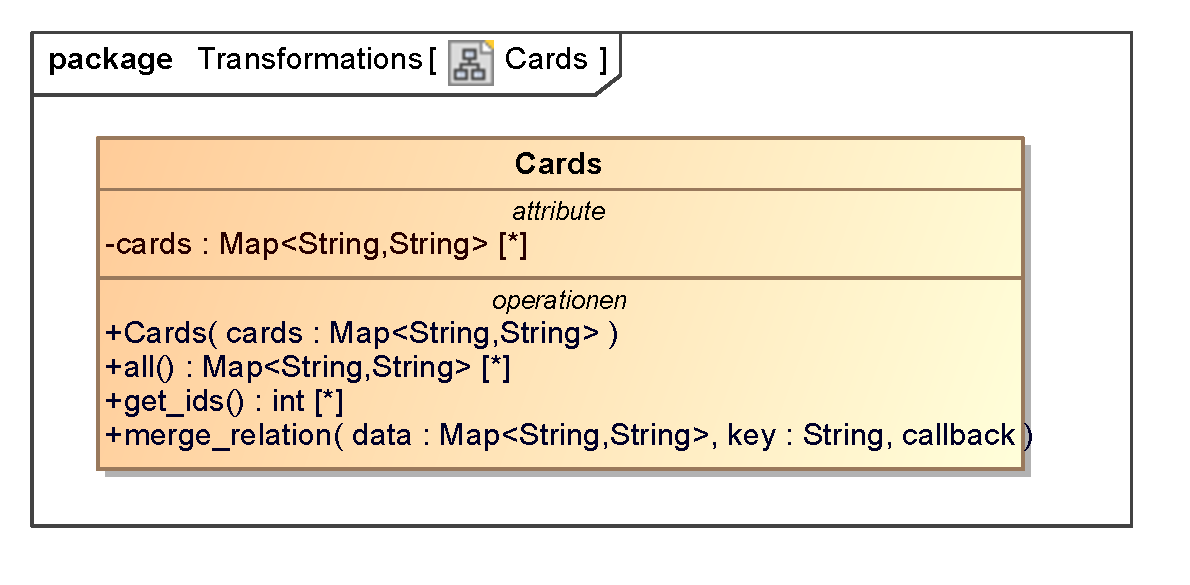
\includegraphics[width=0.75\textwidth]{gfx/MtGDeepAnalysis/Card_Transformations.eps}
    \caption{Klassendiagramm Transformations.Cards}
    \label{fig:class:transformations.cards}
\end{figure}

\begin{description}
    \item[constructor(cards)] \hfill \\
    Speichert die Karten \verb|cards|
    
    \item[all()] \hfill \\
    Ausgabe aller Karten
    
    \item[get\_ids()] \hfill \\
    Gibt eine List von allen Karten-IDs zurück.
    
    \item[merge\_relation(data, key, callback)] \hfill \\
    Fügt die Daten einer Beziehung zu den Karten-Daten hinzu. Die Liste der Argumente befindet sich in \autoref{tab:transformations.cards.merge_relation}
\end{description}

\begin{table}[h]
    \caption{Transformations.Cards::merge\_relation(data : Dictionary[], key : string, callback : Closure)} 
    \myfloatalign
    \begin{tabularx}{\textwidth}{lX}
        \toprule 
        \tableheadline{Eingabe} & \tableheadline{Beschreibung} \\ 
        \midrule 
        \verb|data : Map<String,String>| & Daten der Verknüpfung \\
        \verb|key : string| & Name unter dem die Verknüpfung in den Karten-Daten verfügbar sein soll \\
        \verb|callback : Closure| & Funktion, um Elemente der Verknpüfung zu bearbeiten bevor diese zu den Karten-Daten hinzugefügt werden \\
        \bottomrule 
    \end{tabularx}
    \label{tab:transformations.cards.merge_relation}
\end{table}


%%%%%%%%%%%%%
%% Builder %%
%%%%%%%%%%%%%

\subsubsection{Builder.Builder}
Die Klasse \verb|Builder.Builder| hat die folgenden Schnittstellen:

\begin{figure}[H]
    \myfloatalign
    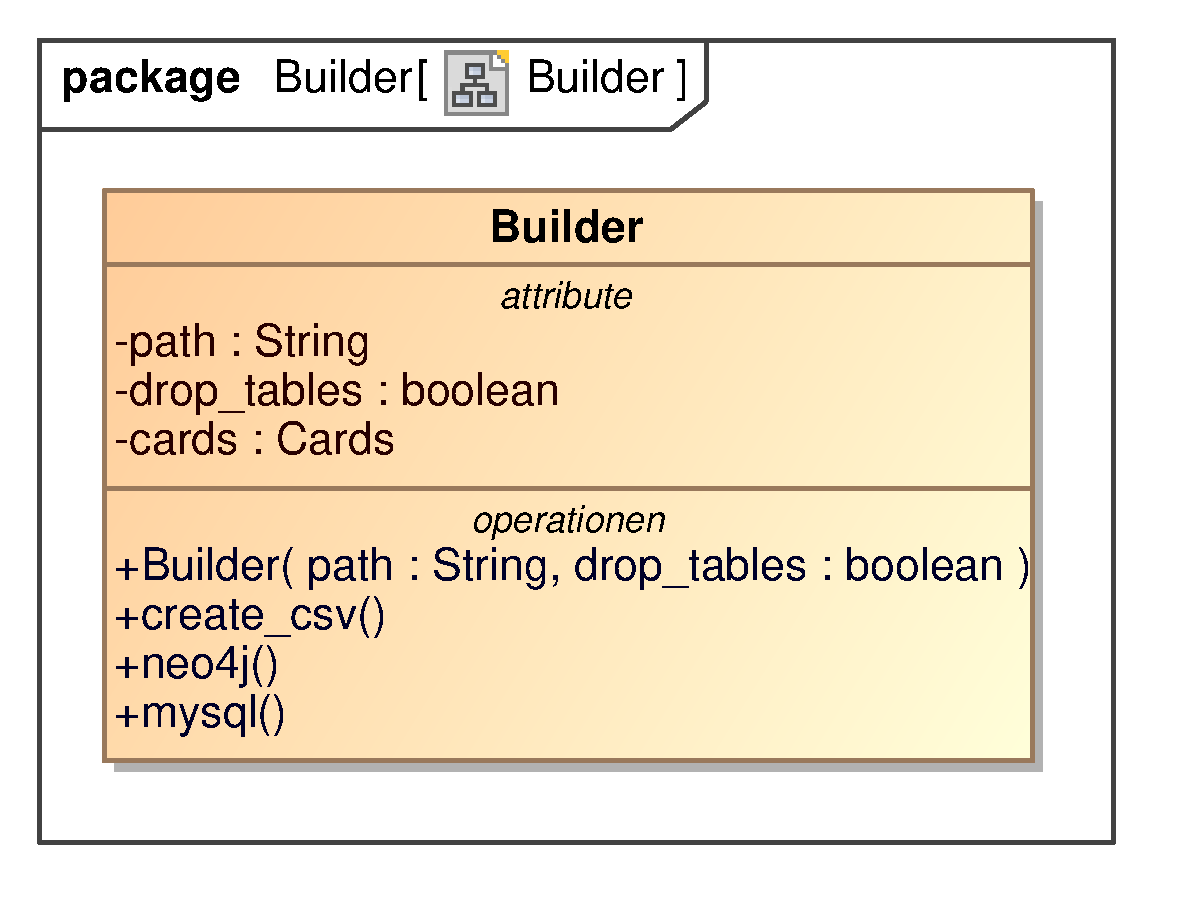
\includegraphics[width=0.65\textwidth]{gfx/MtGDeepAnalysis/Builder.eps}
    \caption{Klassendiagramm Builder.Builder}
    \label{fig:class:builder.builder}
\end{figure}

\begin{description}
    \item[constructor(path, drop\_tables)] \hfill \\
    Einrichten der Datenstruktur \verb|Cards|, speicher des Pfades zur \ac{JSON}-Datei, welche die Karten-Daten enthält
    
    \item[create\_csv()] \hfill \\
    Lädt die Kartendaten aus der \ac{JSON}-Datei und speichert die aufbereiteten Ergebnisse in \ac{CSV}-Dateien
    
    \item[neo4j()] \hfill \\
    Erstellt und befüllt die Neo4j Datenbank mit den Daten aus den \ac{CSV}-Dateien. Löscht alte Daten falls \verb|drop_tables = True|
    
    \item[mysql()] \hfill \\
    Erstellt und befüllt die MySQL Datenbank mit den Daten aus den \ac{CSV}-Dateien. Löscht alte Daten falls \verb|drop_tables = True|
\end{description}

\subsubsection{Builder.CSVHandler}
Die Klasse \verb|Builder.CSVHandler| hat die folgenden Schnittstellen:

\begin{figure}[H]
    \myfloatalign
    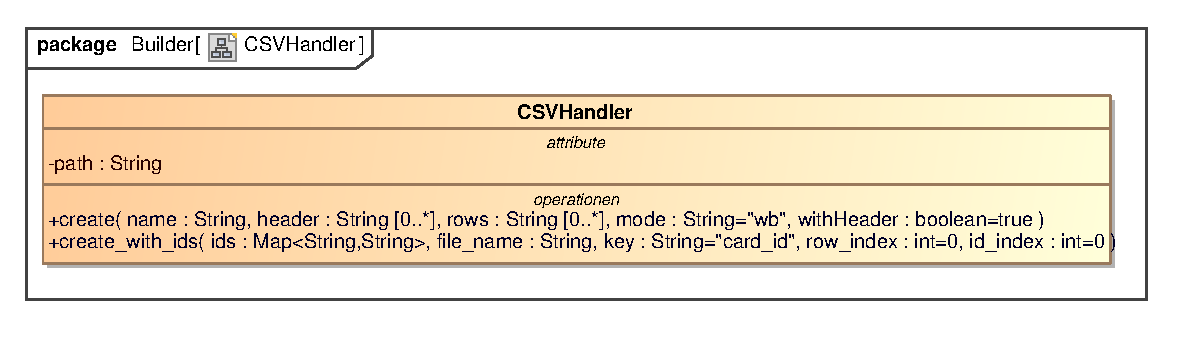
\includegraphics[width=\textwidth]{gfx/MtGDeepAnalysis/CSVHandler.eps}
    \caption{Klassendiagramm Builder.CSVHandler}
    \label{fig:class:builder.CSVHandler}
\end{figure}

\begin{description}
    \item[CSVHandler(path)] \hfill \\
    Speichert Pfadangabe
    
    \item[create(name, header, rows, mode="wb", withHeader=True)] \hfill \\
    Erstellt eine \ac{CSV}-Datei mit dem Namen \verb|name| und dem Header \verb|header| und befüllt diese mit den Reihen \verb|rows|. Mit \verb|mode| kann der Schreibmodus \emph{(überschreiben, anhängen)} angegeben werden und mit \verb|withHeader| ob der \verb|header| hinzugefügt werden soll.
    
    \item[create\_with\_ids(ids, file\_name, key="card\_id", row\_index=0, id\_index=0)] \hfill \\
    Erstellt eine \ac{CSV}-Datei mit dem Namen \verb|file_name| welche die IDs vom Typ \verb|key| hat. \verb|row_index| gibt den Index der CSV Spalte an, die die ID erhält und \verb|id_index| den Index an dessen Stelle die ID sich in \verb|ids| befindet.
\end{description}

\subsubsection{Builder.Cards}
Die Klasse \verb|Builder.Cards| hat die folgenden Schnittstellen:

\begin{figure}[H]
    \myfloatalign
    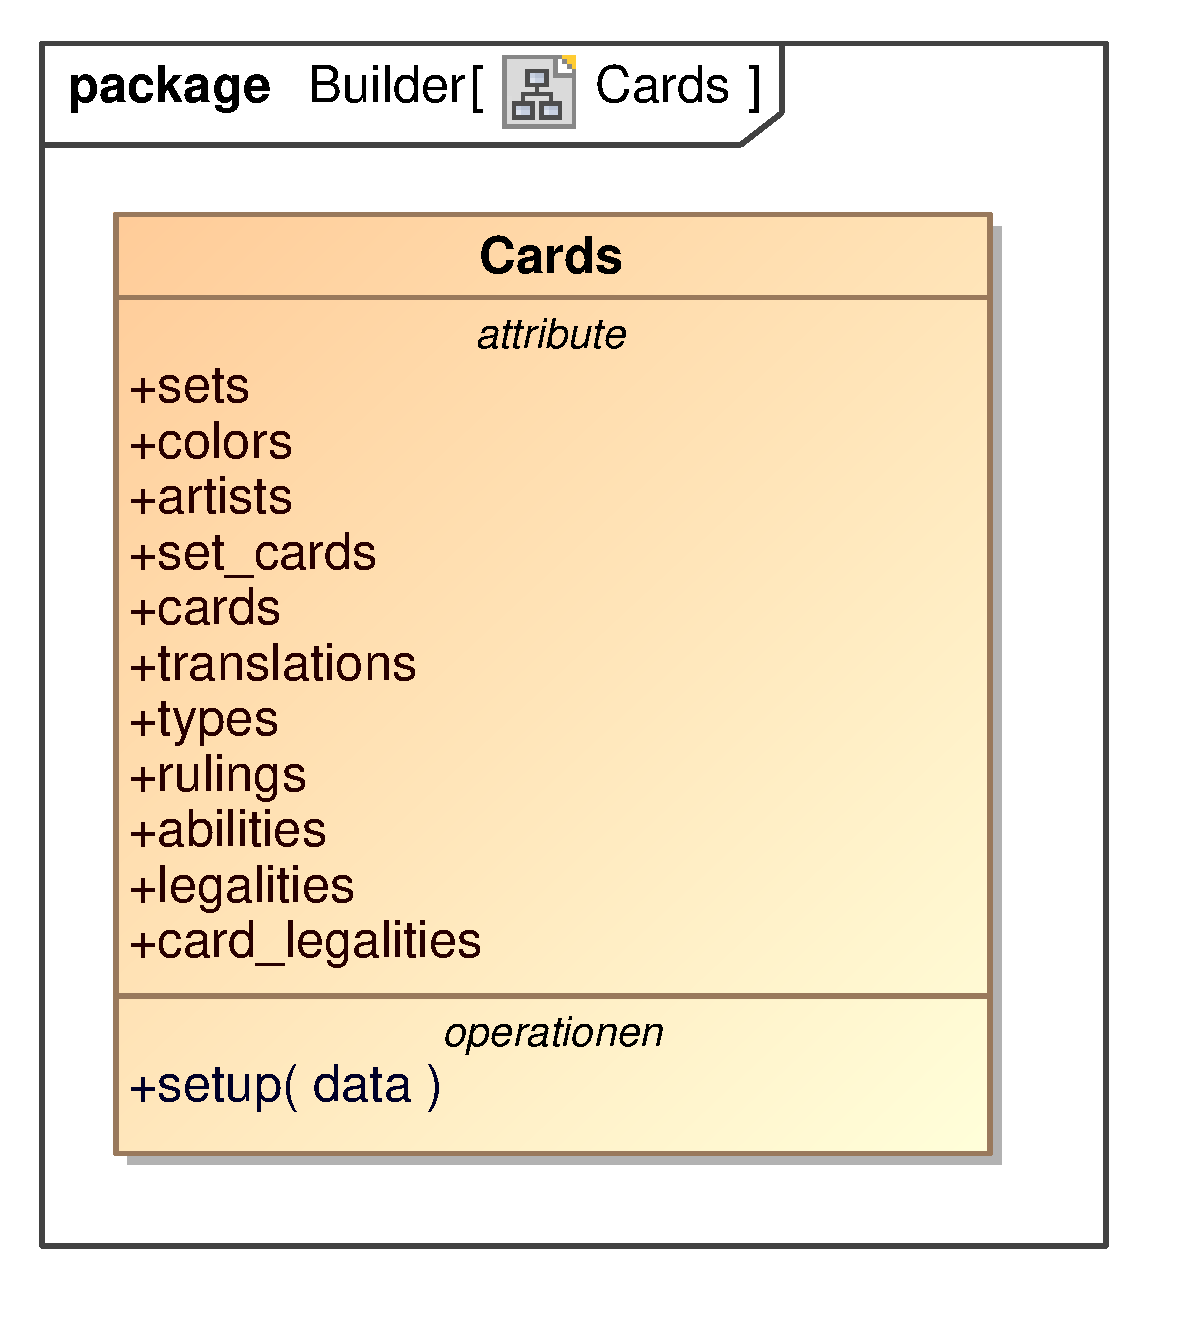
\includegraphics[width=0.5\textwidth]{gfx/MtGDeepAnalysis/Cards.eps}
    \caption{Klassendiagramm Builder.Cards}
    \label{fig:class:builder.cards}
\end{figure}

\begin{description}
    \item[Cards()] \hfill \\
    Erstelle Listen und Daten-Container.
    
    \item[setup(data)] \hfill \\
    Bearbeitet Kartendaten \verb|data|, so dass diese als \ac{CSV}-Dateien gespeichert werden können für den späteren Datenbank-Import.
\end{description}



\subsubsection{Builder.Tournaments}
Die Klasse \verb|Builder.Tournaments| hat die folgenden Schnittstellen:

\begin{figure}[H]
    \myfloatalign
    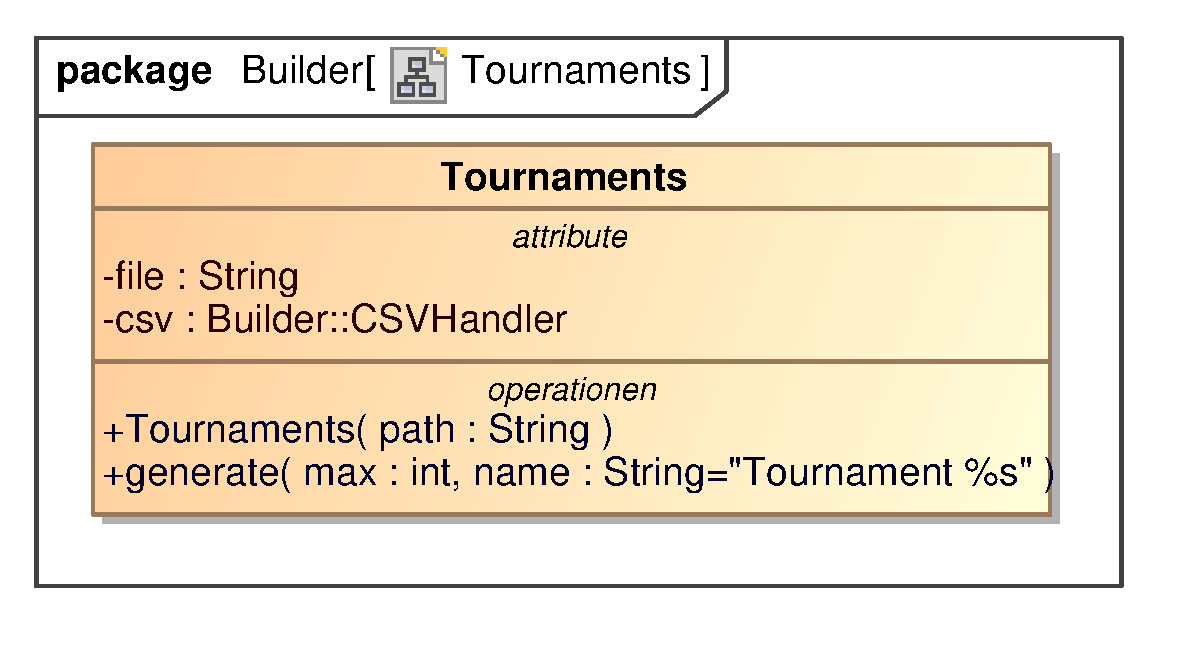
\includegraphics[width=0.65\textwidth]{gfx/MtGDeepAnalysis/Tournaments.eps}
    \caption{Klassendiagramm Builder.Tournaments}
    \label{fig:class:builder.Tournaments}
\end{figure}

\begin{description}
    \item[Tournaments(path)] \hfill \\
      Initiiert den \verb|CSVHandler| mit \verb|path|
     
    \item[generate(max, name="Tournament \%s")] \hfill \\
    Generiere \verb|max| Turniere mit den Namen \verb|name|
\end{description}

\subsubsection{Builder.Scaling}
Die Klasse \verb|Builder.Scaling| hat die folgenden Schnittstellen:

\begin{figure}[H]
    \myfloatalign
    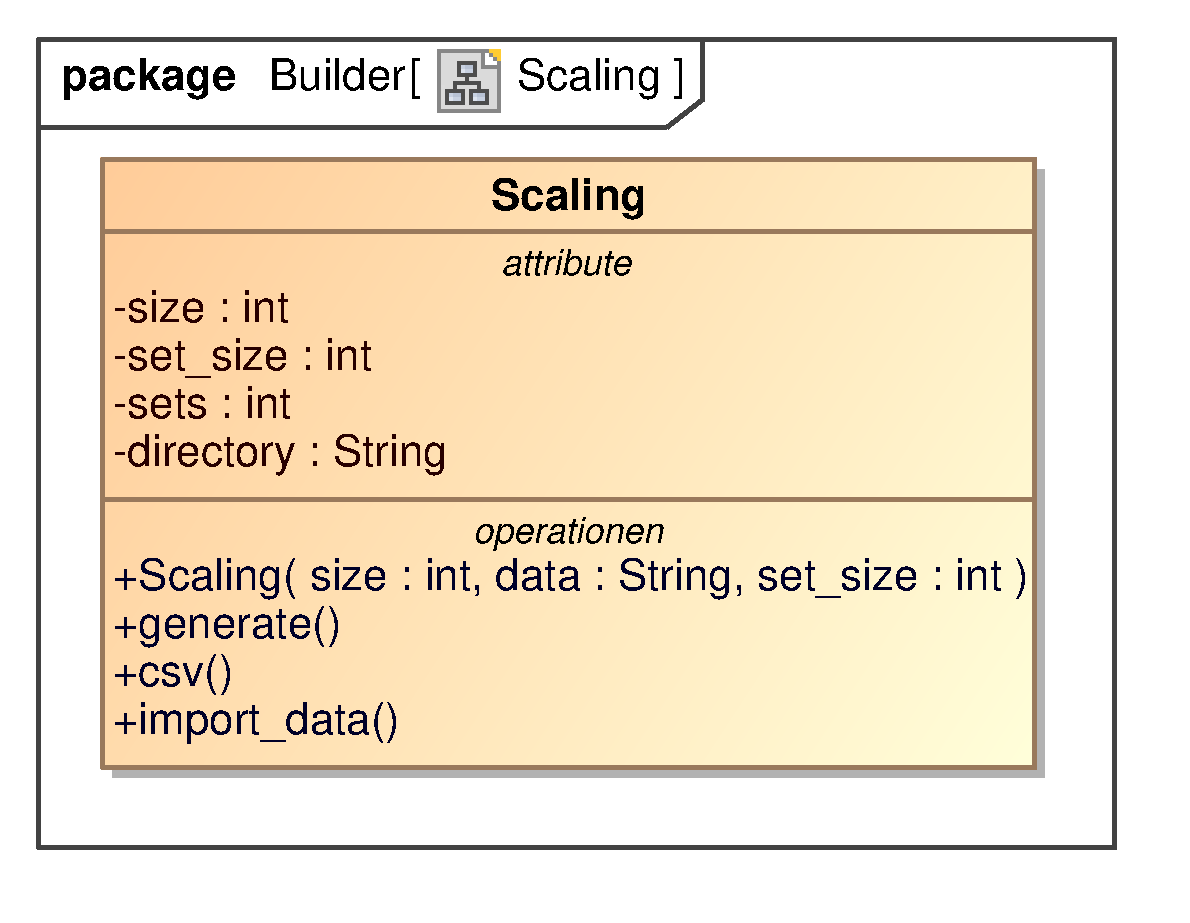
\includegraphics[width=0.65\textwidth]{gfx/MtGDeepAnalysis/Scaling.eps}
    \caption{Klassendiagramm Builder.Scaling}
    \label{fig:class:builder.Scaling}
\end{figure}

\begin{description}
    \item[Scaling(size, data, set\_size=250)] \hfill \\
    Berechne die Anzahl der zu generierenden Sets anhand von \verb|size| und \verb|set_size| und erstelle die nötigen Verzeichnisse in \verb|data|.
    
    \item[generate()] \hfill \\
    Generiere Dummy-Data und speichere diese als \ac{JSON} Dateien
    
    \item[csv()] \hfill \\
    Lade Dummy-Data aus \ac{JSON} Dateien und speichere diese als \ac{CSV} Dateien, sodass sie von der Datenbank importiert werden können
    
    \item[import\_data()] \hfill \\
    Importiere die generierten \ac{CSV} in die beiden Datenbanken
\end{description}


%%%%%%%%%%%%%%%%%%%%%%
%% Builder.Handlers %%
%%%%%%%%%%%%%%%%%%%%%%
\subsubsection{Builder.Handlers.MySQLBuilder}
Die Klasse \verb|Builder.Handlers.MySQLBuilder| hat die folgenden Schnittstellen:

\begin{figure}[H]
    \myfloatalign
    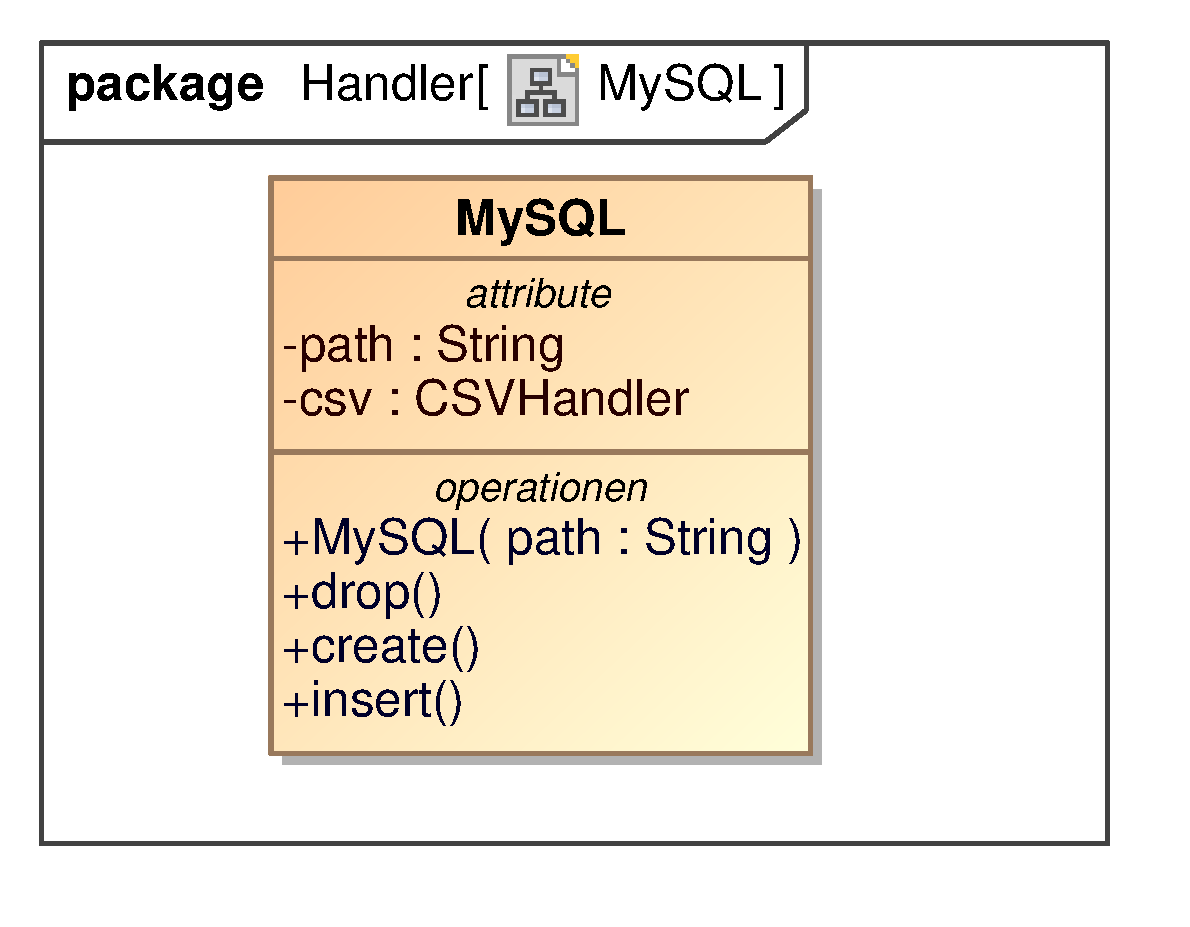
\includegraphics[width=0.5\textwidth]{gfx/MtGDeepAnalysis/MySQL.eps}
    \caption{Klassendiagramm Builder.Handlers.MySQLBuilder}
    \label{fig:class:builder.handlers.mysqlbuilder}
\end{figure}

\begin{description}
    \item[MySQL(path)] \hfill \\
    Initiiere den \verb|CSVHandler| mit \verb|path| und baue die Datenbankverbindung auf.
    
    \item[drop()] \hfill \\
       Löscht Tabellen.
       
    \item[create()] \hfill \\
        Erstellt Tabellen.
        
    \item[insert()] \hfill \\
        Importiert Daten aus den \ac{CSV}-Dateien.
    
    \item[insert()] \hfill \\
        Importiert Dummy-Daten aus den erstellten Skalierungs-CSV-Dateien.
\end{description}


\subsubsection{Builder.Handlers.Neo4jBuilder}
Die Klasse \verb|Builder.Handlers.Neo4jBuilder| hat die folgenden Schnittstellen:

\begin{figure}[H]
    \myfloatalign
    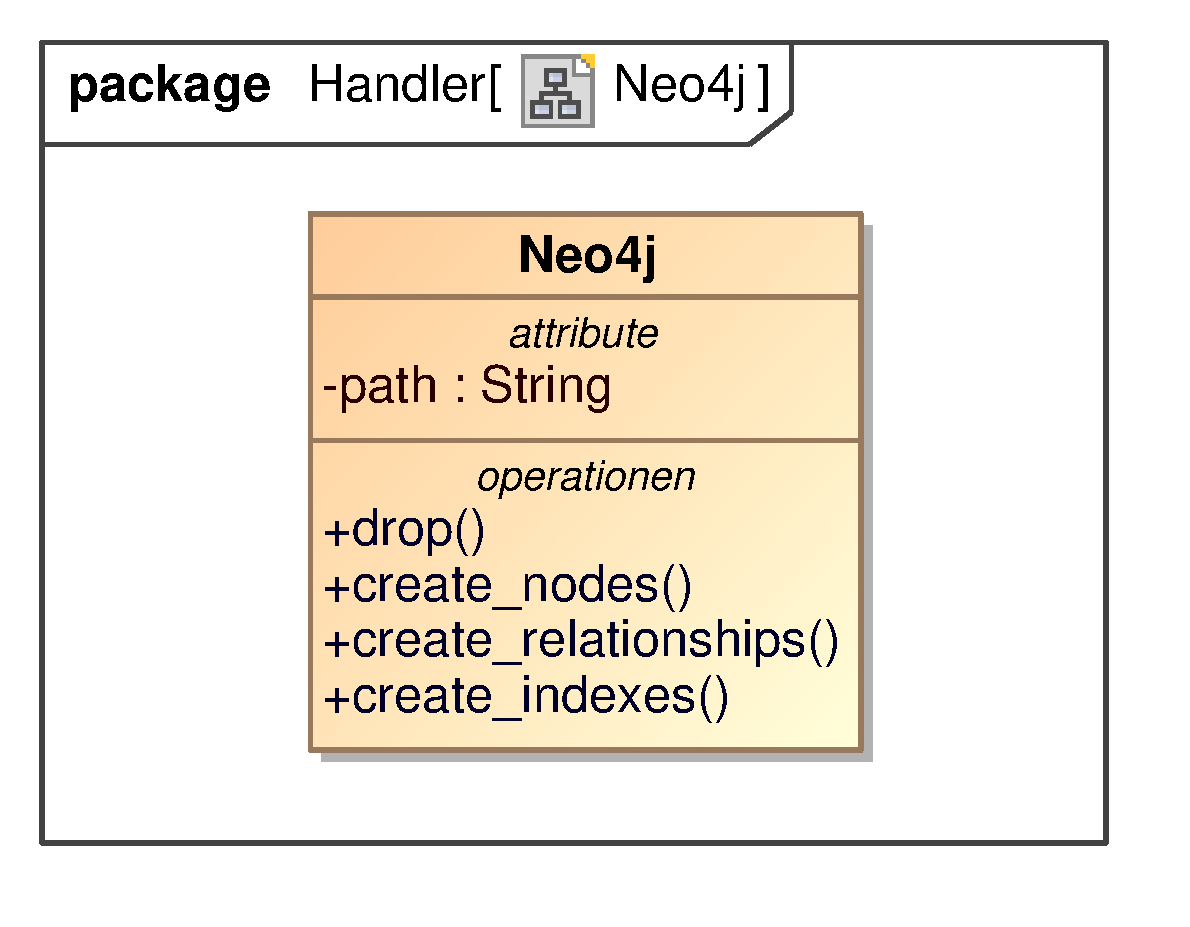
\includegraphics[width=0.5\textwidth]{gfx/MtGDeepAnalysis/Neo4j.eps}
    \caption{Klassendiagramm Builder.Handlers.Neo4jBuilder}
    \label{fig:class:builder.handlers.neo4jbuilder}
\end{figure}

\begin{description}
    \item[constructor(path)] \hfill \\
    Speichere die Pfadangabe \verb|path| zu den \ac{CSV}-Dateien und baue die Datenbankverbindung auf.
    
    \item[drop()] \hfill \\
    Löscht Datenbank.
    
    \item[create\_nodes()] \hfill \\
    Erstellt alle Knoten mit Daten aus den \ac{CSV}-Dateien.
    
    \item[create\_indexes()] \hfill \\
    Erstellt Indizes.
    
    \item[create\_relationships()] \hfill \\
    Erstellen Beziehungen zwischen Daten aus den \ac{CSV}-Dateien.
\end{description}

%%%%%%%%%%%%%%%%%
%% Tournaments %%
%%%%%%%%%%%%%%%%%

\subsubsection{Tournaments.Matches}
Die Klasse \verb|Tournaments.Matches| hat die folgenden Schnittstellen:

\begin{figure}[H]
    \myfloatalign
    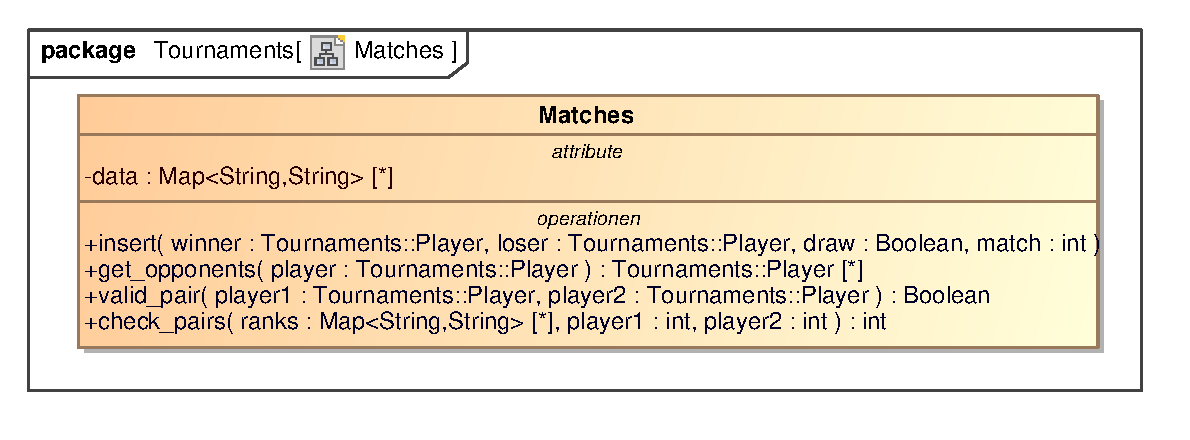
\includegraphics[width=0.95\textwidth]{gfx/MtGDeepAnalysis/Matches.eps}
    \caption{Klassendiagramm Tournaments.Matches}
    \label{fig:class:Tournaments.Matches}
\end{figure}

\begin{description}
    \item[insert(winner, loser, draw, match)] \hfill \\
    Hinzufügen eines neuen Matches
    
    \item[get\_opponents(player)] \hfill \\
    Gibt eine List mit allen bisherigen Gegnern von \verb|player| zurück.
    
    \item[valid\_pair(player1, player2)] \hfill \\
    Überprüft ob eine valide Paarung vorliegt, das heißt die beiden Spieler noch nicht gegeneinander gespielt haben.
    
    \item[check\_pairs(ranks, player1, player2)] \hfill \\
    Überprüft ob eine valide Paarung vorliegt, falls nicht suche rekursiv nach einem möglichen Spieler 2 für \verb|player1|
\end{description}

\subsubsection{Tournaments.Player}
Die Klasse \verb|Tournaments.Player| hat die folgenden Schnittstellen:

\begin{figure}[H]
    \myfloatalign
    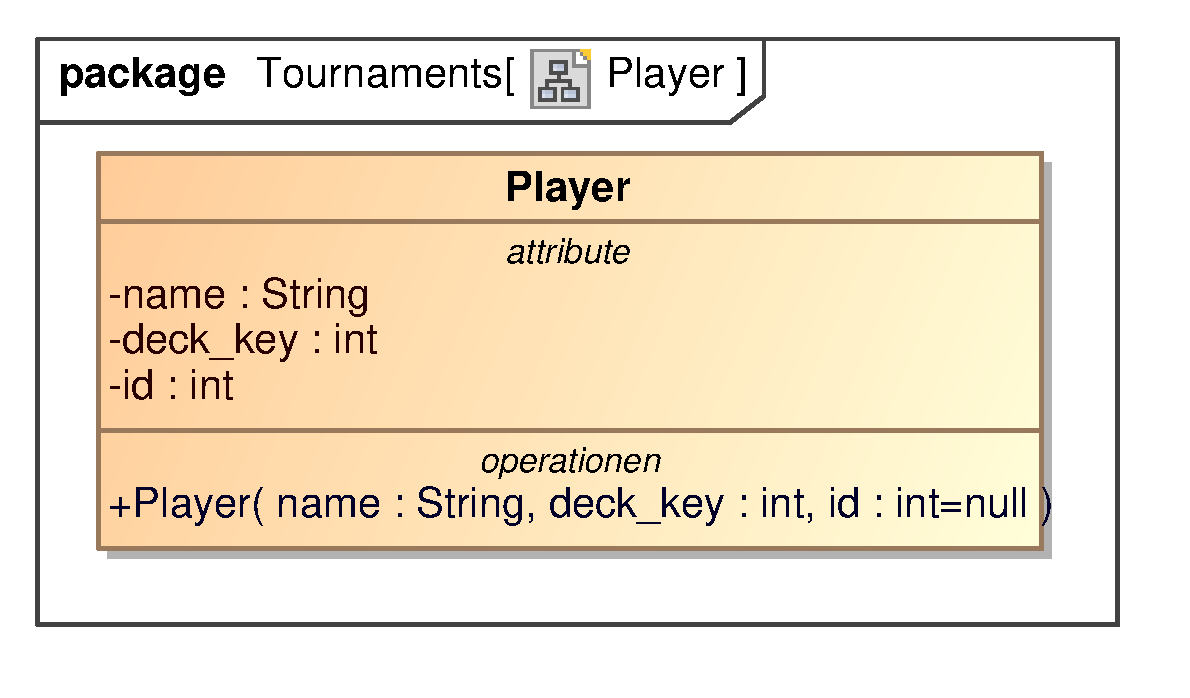
\includegraphics[width=0.65\textwidth]{gfx/MtGDeepAnalysis/Player.eps}
    \caption{Klassendiagramm Tournaments.Player}
    \label{fig:class:Tournaments.Player}
\end{figure}

\begin{description}
    \item[Player(name, deck\_key, id)] \hfill \\
    Anlegen eines Spielers \verb|name| mit der ID \verb|id| \emph{(falls vorhanden)} und dem Deck \verb|deck_key|
\end{description}

\subsubsection{Tournaments.Scoreboard}
Die Klasse \verb|Tournaments.Scoreboard| hat die folgenden Schnittstellen:

\begin{figure}[H]
    \myfloatalign
    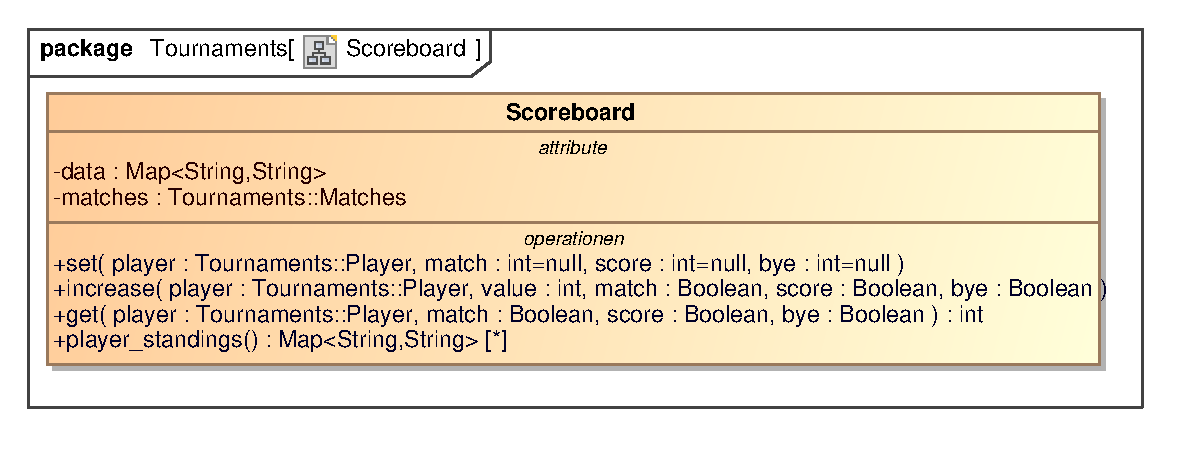
\includegraphics[width=\textwidth]{gfx/MtGDeepAnalysis/Scoreboard.eps}
    \caption{Klassendiagramm Tournaments.Scoreboard}
    \label{fig:class:Tournaments.Scoreboard}
\end{figure}

\begin{description}
    \item[(player, score, match, bye)] \hfill \\
    Setze das Ergebnis, Match oder den Bye eines Spielers \verb|player|
     
    \item[set(player, value, score, match, bye)] \hfill \\
    Erhöhe das Ergebnis, Match oder den Bye eines Spielers \verb|player| um \verb|value|
    
    \item[get(player, score, match, bye)] \hfill \\
    Gibt entweder das Ergebnis, Match oder den Bye eines Spielers \verb|player| zurück
    
    \item[player\_standings()] \hfill \\
    Gibt eine Liste der Spieler und ihrer Gewinn-Historie zurück, sortiert nach Siegen. Der erste Eintrag in der Liste sollte der Spieler an erster Stelle sein
\end{description}

\subsubsection{Tournaments.Tournament}
Die Klasse \verb|Tournaments.Tournament| hat die folgenden Schnittstellen:

\begin{figure}[H]
    \myfloatalign
    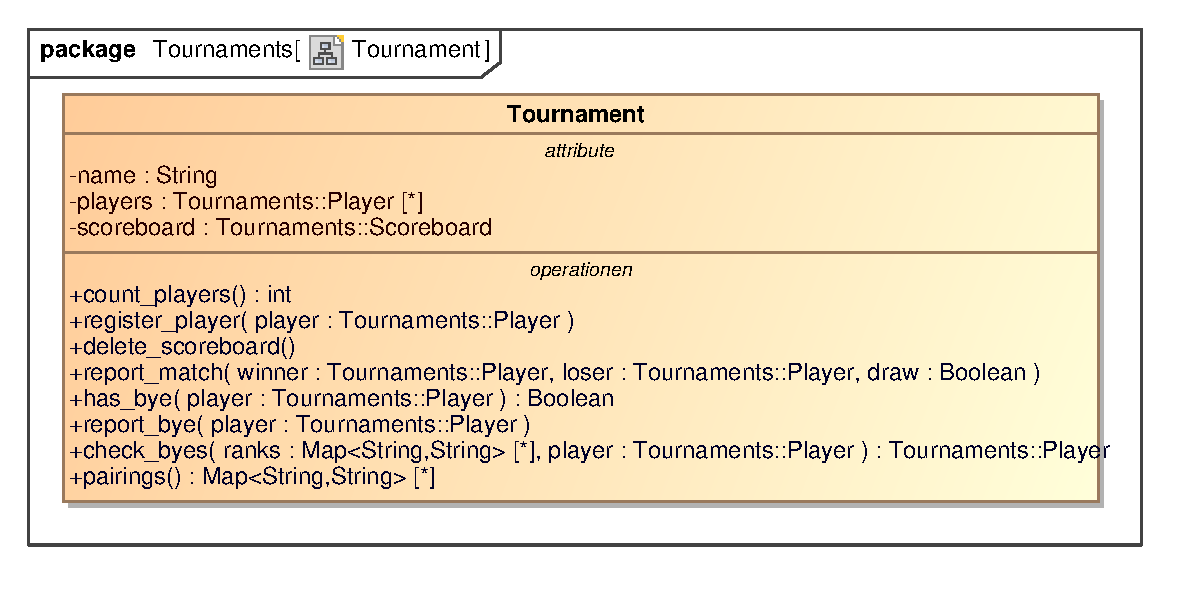
\includegraphics[width=\textwidth]{gfx/MtGDeepAnalysis/Tournament.eps}
    \caption{Klassendiagramm Tournaments.Tournament}
    \label{fig:class:Tournaments.Tournament}
\end{figure}

\begin{description}
    \item[count\_players()] \hfill \\
    Liefert die Anzahl der Spieler des Turniers
    
    \item[register\_player(player)] \hfill \\
    Fügt dem Turnier einen neuen Spieler hinzu
    
    \item[delete\_scoreboard()] \hfill \\
    Löscht Sie das Scoreboard und die Spielerliste
    
    \item[report\_match(winner, loser, draw)] \hfill \\
    Aufzeichnen der Ergebnisse eines einzelnen Spiels zwischen zwei Spielern.
    
    \item[has\_bye(player)] \hfill \\
    Prüft ob der Spieler Bye hat
    
    \item[report\_bye(player)] \hfill \\
    Füge dem Spieler Punkte für einen Bye hinzu
    
    \item[check\_byes(ranks, player)] \hfill \\
    Überprüfe ob der Spieler schon ein Bye hat, falls ja wird der erste Spieler zurückgegeben der noch kein Bye hat
    
    \item[pairings()] \hfill \\
    Gibt eine Liste von Spielernamen für die nächste Runde eines Spiels zurück. Unter der Annahme, dass es eine gerade Anzahl von registrierten Spielern gibt, erscheint jeder Spieler genau einmal in den Paarungen. Jeder Spieler wird mit einem anderen Spieler mit einem gleichen oder fast gleichen Gewinn Rekord gepaart.
\end{description}

%%%%%%%%%%%
%% Faker %%
%%%%%%%%%%%
\subsubsection{Faker.ManaCostProvider}
Die Klasse \verb|Faker.ManaCostProvider| hat die folgenden Schnittstellen:

\begin{figure}[H]
    \myfloatalign
    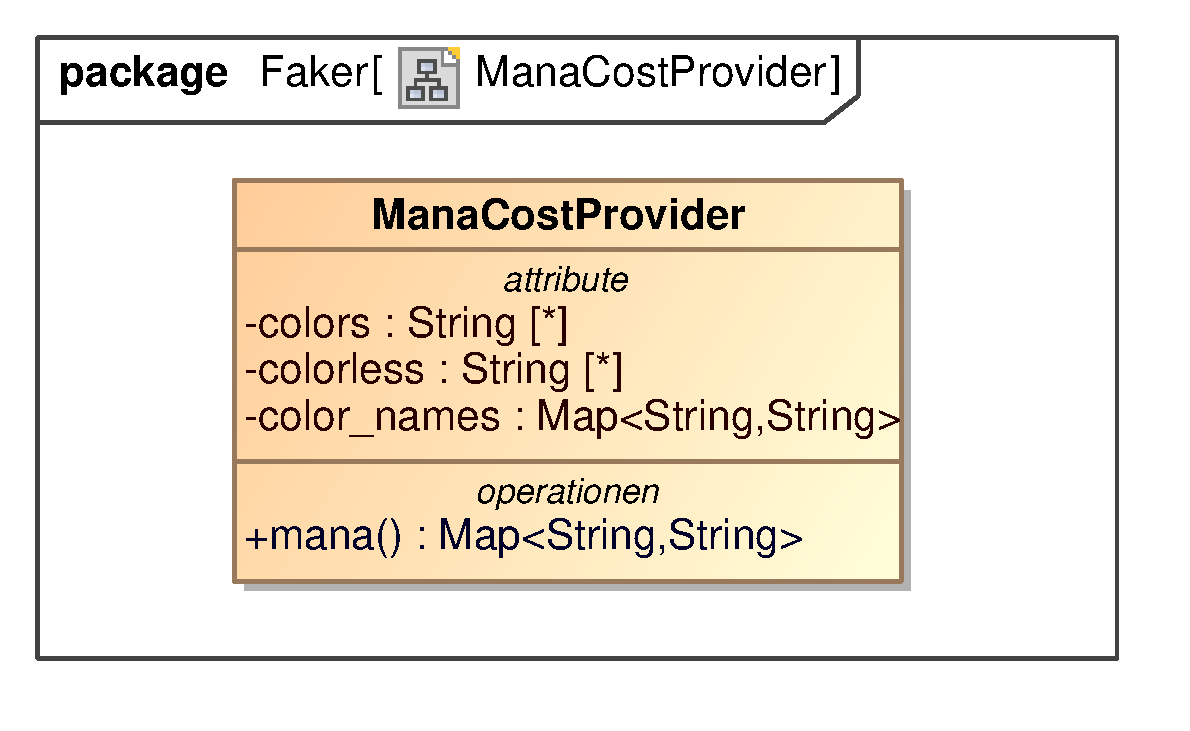
\includegraphics[width=0.6\textwidth]{gfx/MtGDeepAnalysis/ManaCostProvider.eps}
    \caption{Klassendiagramm Faker.ManaCostProvider}
    \label{fig:class:Faker.ManaCostProvider}
\end{figure}

\begin{description}
    \item[mana()] \hfill \\
    Liefert Mana-Kosten, Umgewandelte Manakosten und Farbe zurück
\end{description}

\subsubsection{Faker.TypeProvider}
Die Klasse \verb|Faker.TypeProvider| hat die folgenden Schnittstellen:

\begin{figure}[H]
    \myfloatalign
    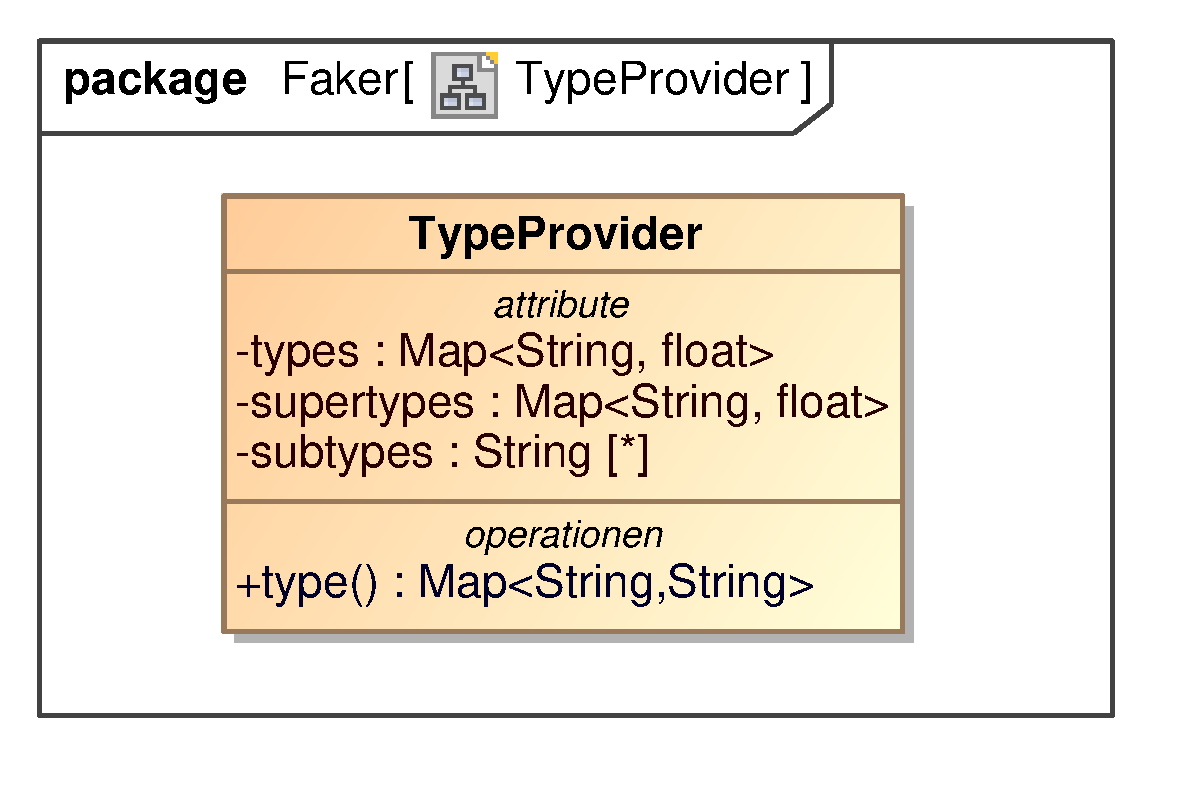
\includegraphics[width=0.6\textwidth]{gfx/MtGDeepAnalysis/TypeProvider.eps}
    \caption{Klassendiagramm Faker.TypeProvider}
    \label{fig:class:Faker.TypeProvider}
\end{figure}

\begin{description}
    \item[type()] \hfill \\
    Liefert Typ, Supertyp und Subtyp zurück
\end{description}

\subsubsection{Faker.CardProvider}
Die Klasse \verb|Faker.CardProvider| hat die folgenden Schnittstellen:

\begin{figure}[H]
    \myfloatalign
    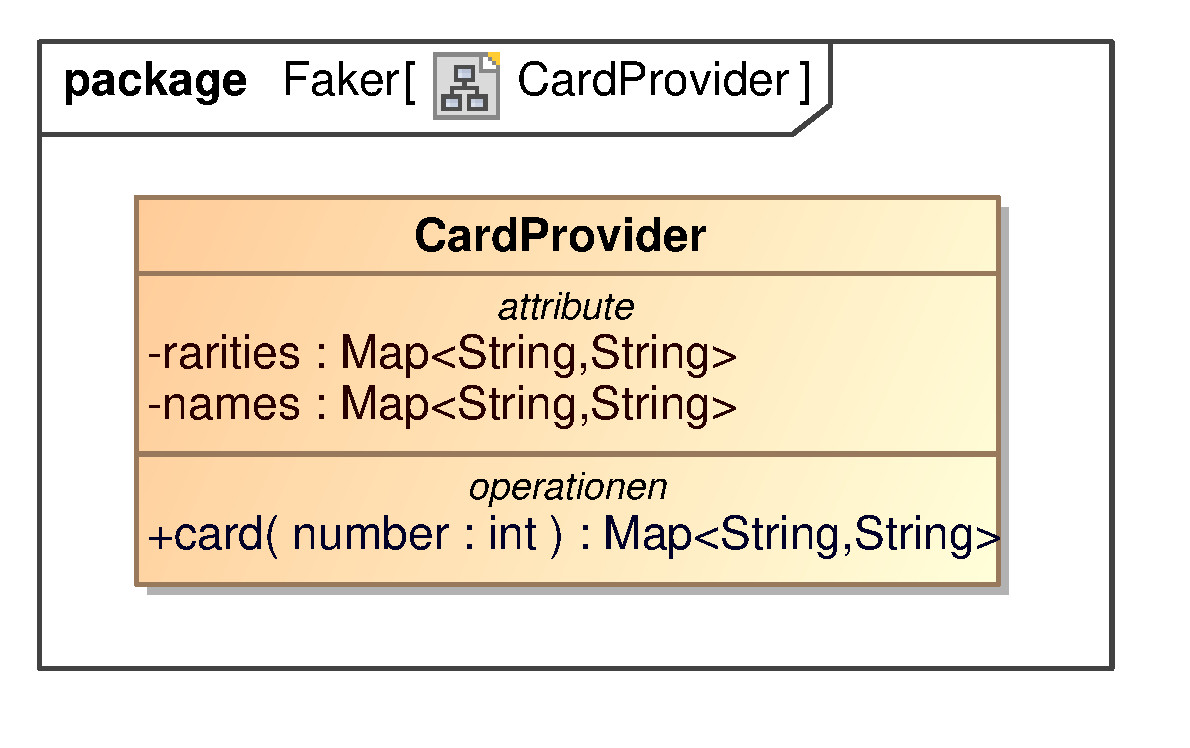
\includegraphics[width=0.6\textwidth]{gfx/MtGDeepAnalysis/CardProvider.eps}
    \caption{Klassendiagramm Faker.CardProvider}
    \label{fig:class:Faker.CardProvider}
\end{figure}

\begin{description}
    \item[card()] \hfill \\
    Liefert Daten zu einer Karte mit Nummber \verb|number| zurück
\end{description}

\subsubsection{Faker.SetProvider}
Die Klasse \verb|Faker.SetProvider| hat die folgenden Schnittstellen:

\begin{figure}[H]
    \myfloatalign
    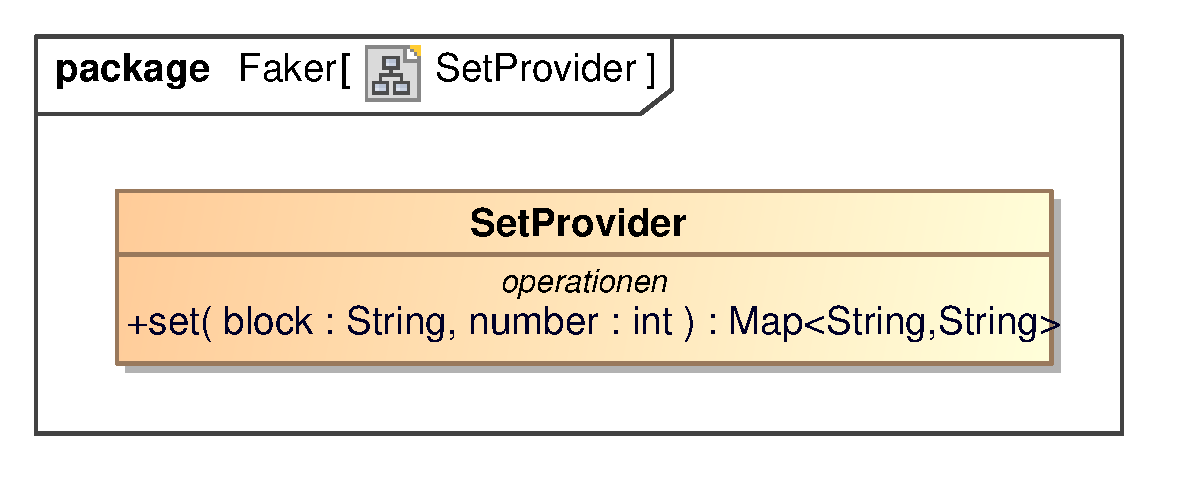
\includegraphics[width=0.6\textwidth]{gfx/MtGDeepAnalysis/SetProvider.eps}
    \caption{Klassendiagramm Faker.SetProvider}
    \label{fig:class:Faker.SetProvider}
\end{figure}

\begin{description}
    \item[card(block, number)] \hfill \\
    Liefert ein Set im \verb|block| Block mit \verb|number| Karten zurück
\end{description}


\subsection{Schnittstellenrealisierung}
%
% Schnittstellenrealisierung -> Interaktionsdiagramm
%
\subsubsection{Fetch} %TODO: Change title
Fetch decks from mtgtop8.com \cite{mtgtop8} %TODO: Change description

\begin{figure}[H]
    \myfloatalign
    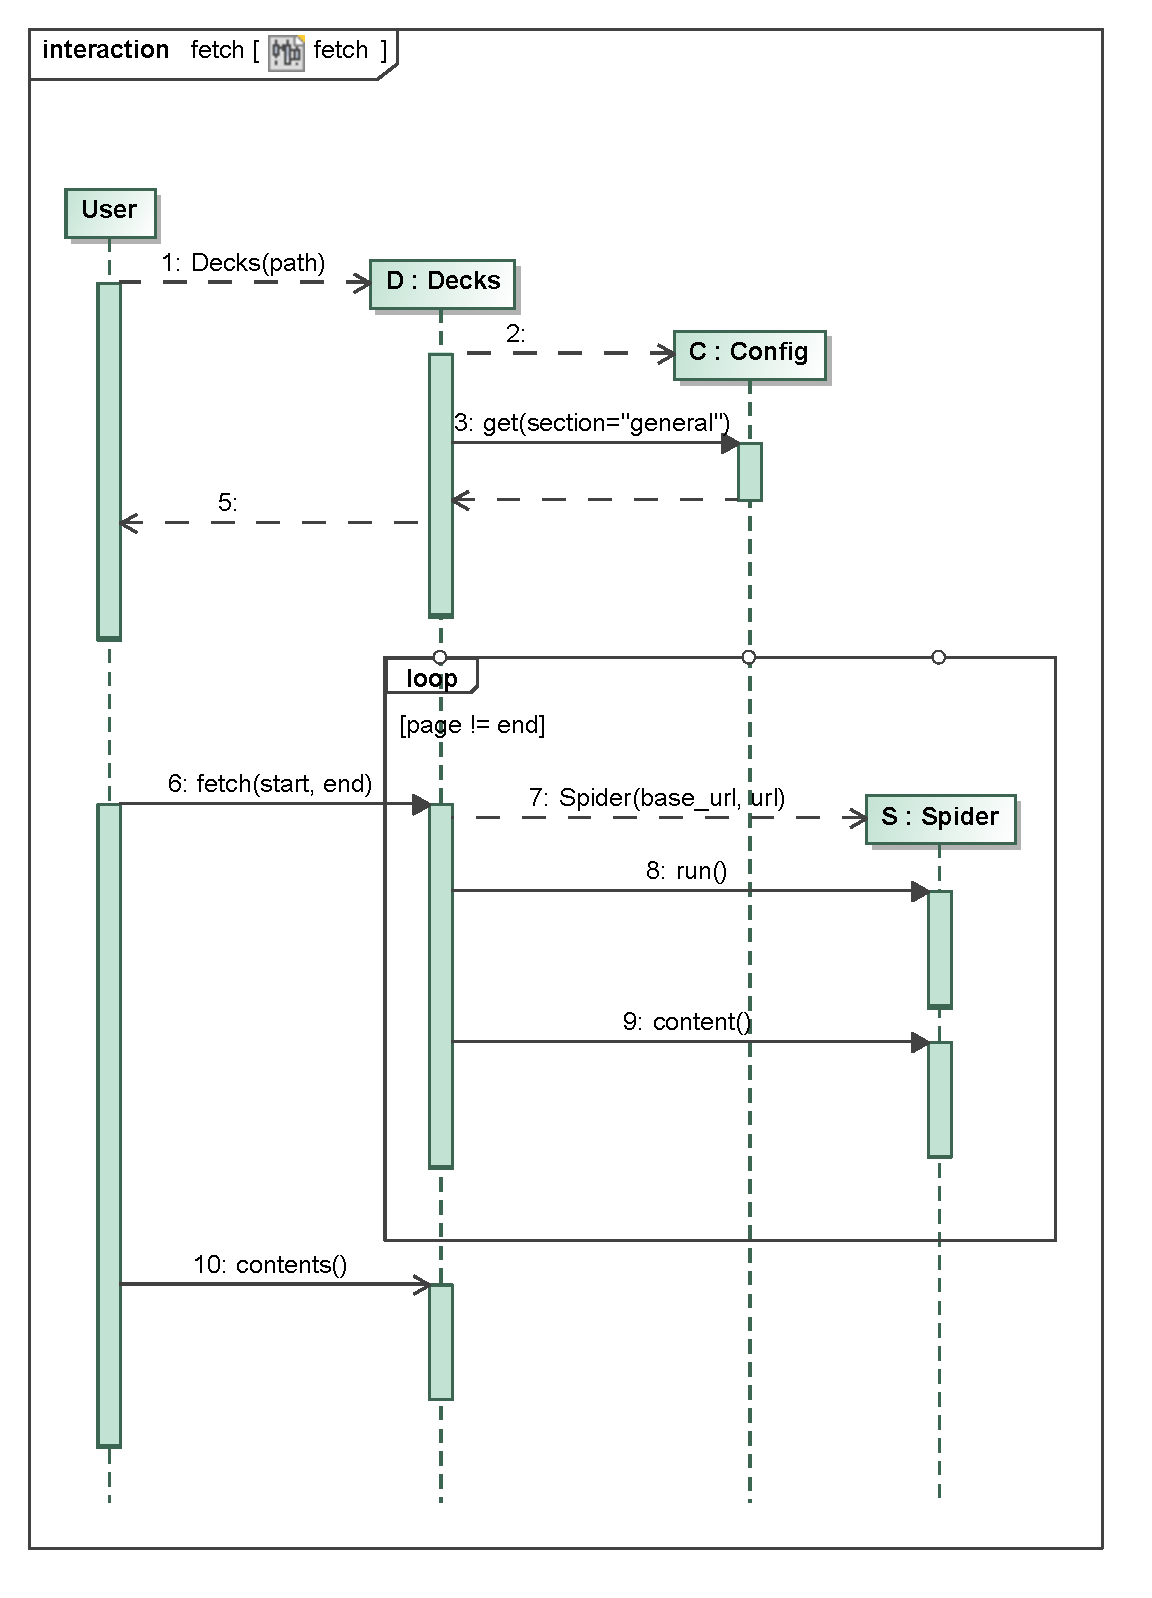
\includegraphics[width=\textwidth]{gfx/MtGDeepAnalysis/fetch.eps}
    \caption{Sequenzdiagramm Fetch} %TODO: Change caption
    \label{fig:seq:fetch}
\end{figure}

\subsubsection{Build} %TODO: Change title
Build \cite{mtgtop8} %TODO: Change description

\begin{figure}[H]
    \myfloatalign
    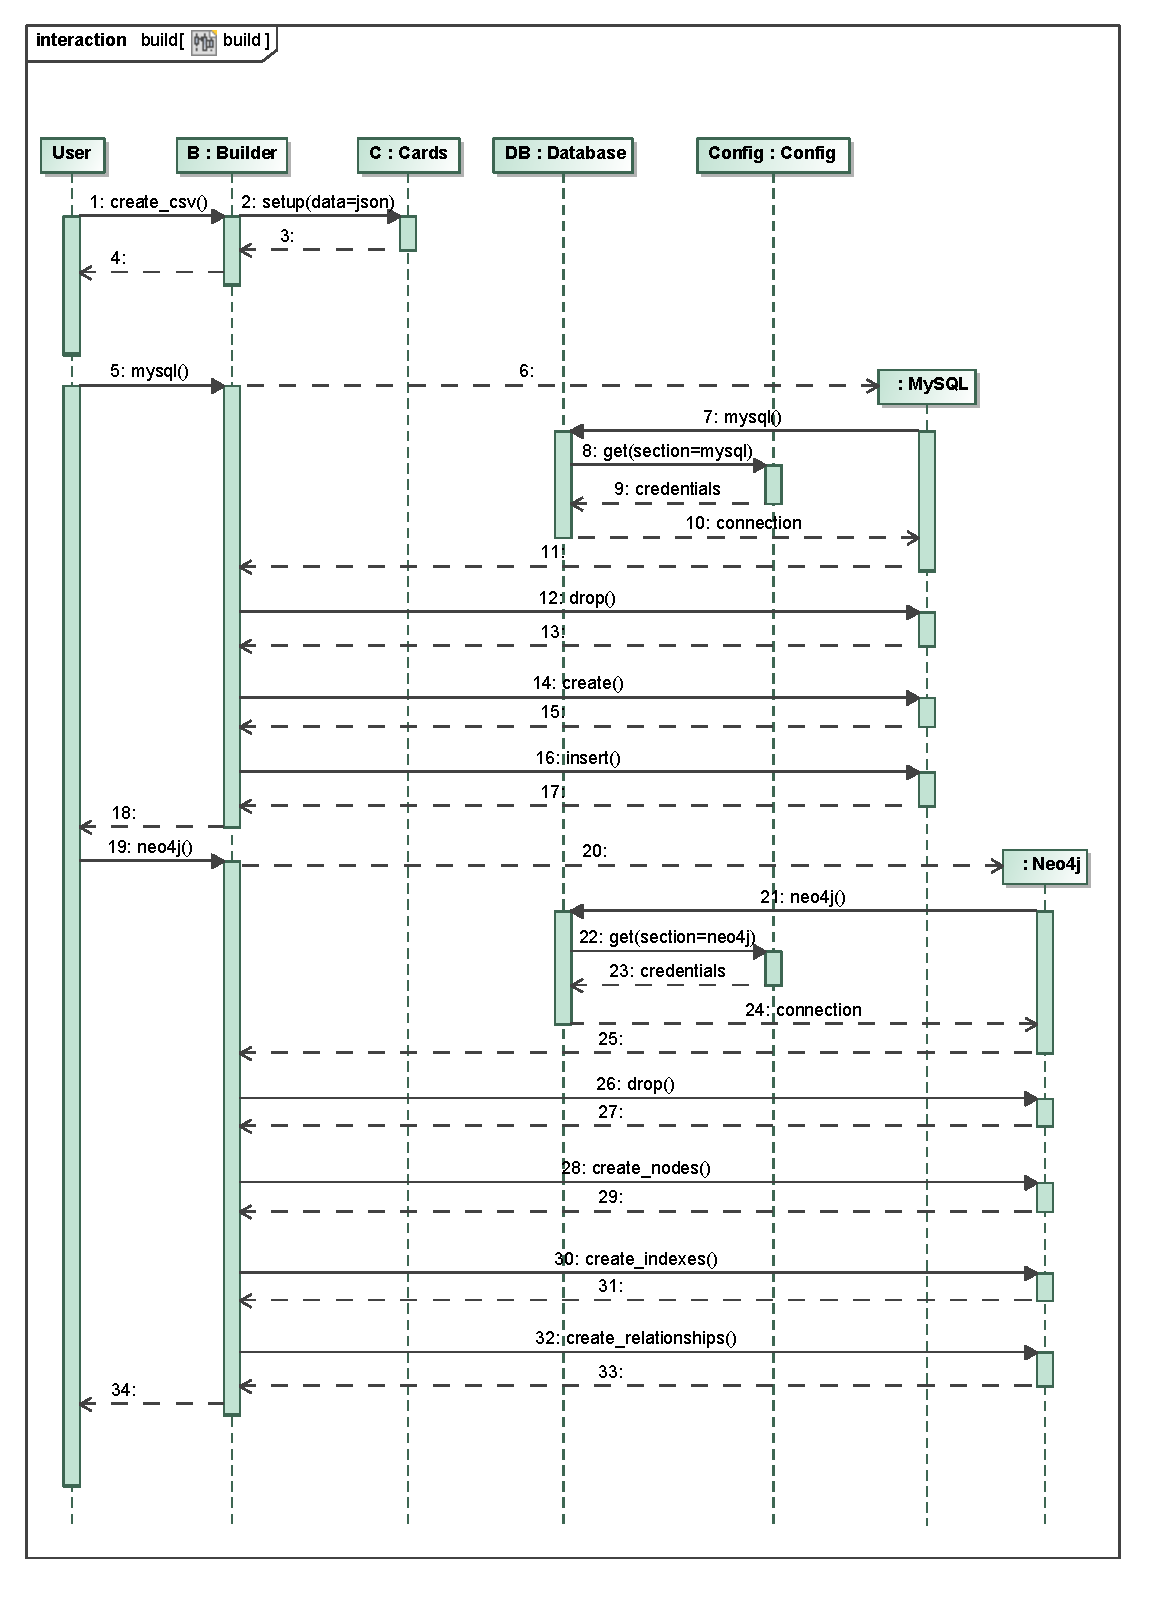
\includegraphics[width=\textwidth]{gfx/MtGDeepAnalysis/build.eps}
    \caption{Sequenzdiagramm build} %TODO: Change caption
    \label{fig:seq:build}
\end{figure}
% !TEX root = ../TUCthesis.tex
%****************************************************
\section{Ausgewählter Ansatz und Detaillösungen}\label{ch:ansatz}
%****************************************************

\subsection{Datenbasis}
Als Basis der Kartendaten wird mtgjson\footnote{http://mtgjson.com} benutzt, welche \ac{MtG} Kartendaten als \ac{JSON} bereitstellt. Die Decks hingegen werden von mtgtop8\footnote{http://mtgtop8.com} bezogen.

\subsection{Datenbanken}
Als Graph-Datenbank wird \emph{Neo4j} eingesetzt, da diese eine hoch skalierbare Datenbank ist, welche auf allen gängigen Betriebssystemen läuft \cite{goel2015neo4j}. Des Weiteren besitzt Neo4j mit \emph{Cypher} eine ausdrucksstarke Abfragesprache. Ein Vorteil von Cypher ist, dass ab Neo4j 2.1 der Import aus \ac{CSV}-Dateien unterstützt wird. \cite{panzarino2014cypher}

%TODO: MariaDB/MySQL
Als \ac{RDBMS} wird MariaDB\footnote{https://mariadb.com} eingesetzt, welche vom Urheber von MySQL entwickelt wird. MariaDB ist ein Fork von MySQL und gilt als dessen evolutionäre Nachfolger. \cite{bartholomew2013getting}

\subsubsection{Import der Daten}
Da eine große Menge an Daten importiert werden müssen, zum Beispiel über 90.000 Übersetzungen, ist eine schnelle Import-Funktion hilfreich. In \autoref{listing:cypher.import.csv} befindet sich ein Kommando, um Übersetzungen nach Neo4j zu importieren und in \autoref{listing:sql.import.csv} ein Kommando, um nach MySQL zu importieren.

\begin{listing}[H]
    \caption{Importieren von Übersetzungen}
    \label{listing:cypher.import.csv}
    \begin{lstlisting}[language=SQL]
    USING PERIODIC COMMIT 1000
    LOAD CSV WITH HEADERS FROM "file:translations.csv" AS row
    CREATE (:Translation { name: row.name });
    \end{lstlisting}
\end{listing}

\begin{listing}[H]
    \caption{Importieren von Übersetzungen}
    \label{listing:sql.import.csv}
    \begin{lstlisting}[language=SQL]
    LOAD DATA LOCAL INFILE 'translations.csv' INTO TABLE `translations`
    CHARACTER SET UTF8
    FIELDS TERMINATED BY ','
    ENCLOSED BY '"'
    LINES TERMINATED BY '\r\n'
    IGNORE 1 LINES
    SET (@card, name, lang, card_id);
    \end{lstlisting}
\end{listing}

\subsection{Programmiersprache}
Als Programmiersprache wird \emph{PyPy}\footnote{http://pypy.org}, eine alternative \emph{Python} Implementierung, verwendet. Die Vorteile von PyPy sind der integrierte \ac{JIT} Compiler, wodurch sich eine schnellere Ausführungszeit ergibt, und der geringere Speicherverbrauch. \cite{doglio2015mastering} 

\subsubsection{Profiling}
Mit einem \emph{Profiler} können verschiedene Werte wie \emph{Ausführungszeit} oder \emph{Speicherverbrauch} gemessen werden \cite{doglio2015mastering}. Um vergleichen zu können, wie gut die Datenbanksysteme in den einzelnen Testfällen abschneiden, werden die Ausführungszeit und der Speicherverbrauch gemessen. 

Für die Ausführungszeit kann eine einfache Timer-Klasse\footnote{https://www.huyng.com/posts/python-performance-analysis} benutzt werden. Um den Speicherverbrauch zu messen wird die Python-Bibliothek psutil benutzt\footnote{http://fa.bianp.net/blog/2013/different-ways-to-get-memory-consumption-or-lessons-learned-from-memory\_profiler/}, da diese eine einfache und plattformübergreifende Methode bietet den Speicherverbrauch auszulesen.
 %%% Evtl aufspalten in "Analyse" und "Design und Realisierung"
% !TEX root = ../TUCthesis.tex
%************************************************
\chapter{Ergebnisse}\label{ch:ergebnisse}
%************************************************
\section{Validierung des Gesamtkonzeptes}

%%%%%%%%%%%%%%%%%%%%%%%%%%%%%%%%%%%%%%%%%%%%%%%%%%%%%%%%%%%%%%%%%%%%%%%%%%%%%%%%%%%%%%%%%%%%%%%%%%%%%
% Testfälle und Beziehung zu Problemen aus Kapitel 3
%
% Eine oftmals hilfreiche Form, die Inhalte dieses Kapitels zu veranschaulichen, ist eine Tabelle,
% welche die Requirements / die Probleme aus Kapitel 3 und die Tests / Ergebnisse aus Kapitel
% 4 zuordnet. Aus dieser Tabelle ist dann ersichtlich, welche Teile abgedeckt, getestet, nicht
% testbar, erwartungsgemäß, abweichend etc. sind.
%
%
% Gesetz der Großen Zahlen, Varianz, Standardabweichung
%%%%%%%%%%%%%%%%%%%%%%%%%%%%%%%%%%%%%%%%%%%%%%%%%%%%%%%%%%%%%%%%%%%%%%%%%%%%%%%%%%%%%%%%%%%%%%%%%%%%
\begin{table}[t]
    \caption{Erforderliche Testfälle} 
    \myfloatalign
    \begin{tabularx}{\textwidth}{lX}
        \toprule 
        \tableheadline{Anforderung} & \tableheadline{Testfall} \\ 
        \midrule 
        Kartensuche: Schlüsselwort-Fähigkeit & Suche alle Karten mit einer bestimmten Fähigkeit \\
        Kartensuche: Textsuche & Suche nach einer Zeichenkette die in einem Kartennamen vorkommt\\
        Kartensuche: Verknüpfungen & Suche anhand verschiedener Karten-Attribute \\
        Turnier: Matchup Analyse & Berechne das Matchup eines Deck-Typen \\
        Turnier: Top 10 Decks & Berechne die 10 besten Decks \\
        \bottomrule 
    \end{tabularx}
    \label{tab:req.tests}
\end{table}
In \autoref{tab:req.tests} befindet sich eine Auflistung der Probleme die in \autoref{ch:analyse} beschrieben wurden und welche Testfälle erforderlich sich, um die Anforderung zu überprüfen.

Jeder Test wurde 1000mal sowohl auf Neo4j als auch auf MySQL/MariaDB ausgeführt, um den Einfluss von Messfehlern zu reduzieren \emph{(Gesetz der Großen Zahlen)}. Bei jedem Test wurde die Ausführungszeit in Millisekunden (ms) und der Speicherverbrauch in MByte gemessen. Um sicherzugehen, dass Caching oder Systemprozesse die Ergebnisse nicht beeinflussen, wurden die 10 längsten und kürzesten Zeiten verworfen. Die übriggebliebenen Werte wurden gemittelt und die Standardabweichung wurde berechnet, um zu schauen wie groß die Fehlergrenzen sind. 

Um zu erfahren wie gut die beiden Datenbanken skalieren, wurden außerdem die Testfälle stückweise auf größeren Datensätzen ausgeführt. Diese Datensätze wurden zufällig generiert und basieren nicht auf echten Daten. Als Staffelung für die Tests wurden \emph{100.000, 250.000, 500.000 und 1.000.000} Karten gewählt.

\section{Beschreibung und Motivation der Testfälle}
%% Tests in normaler Sprache:
%% zB: Testfall X: Suche nach allen Karte die aus Set Y sind und Kriterium Z erfüllen
%%  -> guter test, da viele Verknpüfungen

\subsection{Testfall 1: Schlüsselwort-Fähigkeit}
Eine einfache Suche, um die ersten 300 Karten mit dem Schlüsselwort-Fähigkeit \emph{Flying} zu erhalten. Wie in \autoref{fig:uml:schema} zu sehen ist, werden die Fähigkeiten in MySQL/MariaDB in einer eigenen Tabelle gespeichert. In Neo4j hingegen können diese als Attribut von \emph{Card} hinterlegt werden \emph{(siehe \autoref{fig:graph:schema})}, da Neo4j den Datentyp \emph{Array} unterstützt. Mit diesem Test lässt sich also vergleichen wie gut sich Arrays im Vergleich zu \verb|JOINS| beim durchsuchen eignen.
    
\subsection{Testfall 2: Textsuche}
Eine einfache Suche nach den Karten, die den Namen \emph{Forest} enthalten und die entweder von \emph{Aleksi Briclot} oder \emph{John Avon} gezeichnet wurden. Da Karten anhand ihres Namens identifiziert werden, ist es sinnvoll zu testen wie gut sich eine Textsuche in den beiden Datenbanksystemen funktioniert.

\subsection{Testfall 3: Verknüpfungen}
Eine komplexe Suche nach Karten, welche bestimmte Kriterien erfüllen \emph{(siehe \ref{listing:complex.sql})}. Es wird nach Karten gesucht, die folgende Eigenschaften erfüllen:
\begin{itemize}
    \item in einem Set nach dem \emph{01.01.2001} erschienen
    \item als Seltenheit \emph{RARE} besitzen
    \item in \emph{deutscher} Sprache erschienen
    \item als Farbe \emph{Blau} haben
    \item vom Typ \emph{Kreatur} sind
    \item die Fähigkeit \emph{Flying} besitzen
    \item umgewandelte Manakosten von \emph{maximal 5} haben
 \end{itemize} 

\subsection{Testfall 4: Matchup Analyse}
Berechnung des Matchup für den Deck-Typ \emph{Bant}. Es werden alle Matches analysiert an denen ein Deck vom Typ \emph{Bant} beteiligt war und überprüft ob das Deck gewonnen oder verloren hat. Die Ergebnisse werden dann anhand der gegnerischen Deck-Typen gruppiert und geordnet. Insgesamt gibt es im Standard-Testfall 1000 Turniere mit etwas über 6500 Decks, die jeweils zwischen 2 und 6 Matches enthalten.  

\subsection{Testfall 5: Top 10 Decks}
Für jedes Deck wird das Verhältnis zwischen den gewonnen und verlorenen Matches berechnet und dann der Größe nach sortiert und die ersten 10 Decks gewählt. Je höher der Wert ist, desto besser ist das Deck unabhängig von der Anzahl der gespielten Partien. Insgesamt gibt es im Standard-Testfall 1000 Turniere mit etwas über 6500 Decks, die jeweils zwischen 2 und 6 Matches enthalten. 

\section{Übersicht und Bewertung der erzielten Ergebnisse}
%%
%% Graphen! + Berwertung (erwaret/unwartet, weil | DB X besser geeignet weil)
%%
\subsection{Laufzeit}
Die gemessenen Laufzeiten samt ihrer Standardabweichung sind in \autoref{fig:plot.runtime} als Fehlerbalkendiagramm dargestellt. Wie zu erwarten war ist Neo4j in Testfall 4 schneller als die SQL-Abfrage mit \verb|JOINS|. Überraschenderweise war Neo4j auch in Testfall 2 etwas schneller als MySQL/MariaDB, obwohl aufgrund der langjährigen Optimierungen der Textsuche in MySQL/MariaDB zu erwarten war, dass diese schneller sei. Der Grund dafür, dass Neo4j in den Testfällen 1 und 3 langsamer ist als MySQL/MariaDB liegt vermutlich daran, dass als Datentyp Arrays für \emph{color}, \emph{abilities} und \emph{types} benutzt wurden. Anscheinend ist in Neo4j die Suche innerhalb eines Arrays langsamer als die Suche mit einem \verb|JOIN| in SQL.

\begin{figure}[t]
    \myfloatalign
    \begin{tikzpicture} 
        \begin{axis}[
            width=0.75*\linewidth, % Scale the plot to \linewidth
            grid=major, % Display a grid
            grid style={dashed,gray!30}, % Set the style
            xlabel=Testfälle, % Set the labels
            ylabel=Laufzeit,
            use units,
            y unit=ms,
            %legend style={at={(0.5,-0.2)},anchor=north}, % Put the legend below the plot        
            legend pos=north west,
            enlarge y limits={upper,value=0.15},
            ybar,
            symbolic x coords={Test 1, Test 2, Test 3, Test 4, Test 5},
            xtick=data,
            nodes near coords,
            every node near coord/.append style={rotate=90, anchor=west}
        ]
            \addplot+[error bars/.cd,y dir=both,y explicit]
            table[x=Test,y=Neo4j,y error=Neo4j error,col sep=comma]{evaluation-results/testcases-runtime.n-1000.csv};
            
            \addplot+[error bars/.cd,y dir=both,y explicit]
            table[x=Test,y=MySQL,y error=MySQL error,col sep=comma]{evaluation-results/testcases-runtime.n-1000.csv};
            
            \legend{Neo4j, MySQL/MariaDB}
        \end{axis}
    \end{tikzpicture}
    \caption{Ausführungszeit der einzelnen Testfälle}
    \label{fig:plot.runtime}
\end{figure}

%\begin{table}[t]
%    \caption{Gemessene Laufzeiten der Testfälle} 
%    \myfloatalign
%    \csvreader[tabular=lrrrr,table head=\toprule Test & Neo4j (ms) & Neo4j STD (ms) & MySQL (ms) & MySQL STD (ms) \\\midrule,late after last line=\\\bottomrule]%
%    {evaluation-results/testcases-runtime.n-1000.csv}{Test=\test,Neo4j=\neo,Neo4j error=\neostd,MySQL=\mysql,MySQL error=\mysqlstd}%
%    {\test & \neo & \neostd & \mysql & \mysqlstd}%
%    \label{tab:runtime}
%\end{table}

\subsection{Skalierbarkeit}
Wie in \autoref{fig:plot.scaling.testcase1} zu sehen ist, skalieren sowohl Neo4j als auch MySQL/MariaDB gut, aber auch hier zeigt sich, dass Neo4j in allen gemessenen Punkten langsamer ist. Die Steigung ist bei beiden Datenbanken ungefähr gleich. Die Vermutung, dass die Suche in Arrays langsamer ist als mit \verb|JOINS| bestätigt sich in Testfall 3.

\begin{figure}[t]
    \myfloatalign
    \begin{tikzpicture} 
    \begin{axis}[
    width=0.70*\linewidth, % Scale the plot to \linewidth
    grid=major, % Display a grid
    grid style={dashed,gray!30}, % Set the style
    xlabel=\# Karten, % Set the labels
    ylabel=Laufzeit,
    use units,
    y unit=ms,
    legend pos=north west,
    ]
    \addplot+[color=blue, mark=*,error bars/.cd,y dir=both,y explicit]
    table[x=Size,y=Neo4j,y error=Neo4j error,col sep=comma]{evaluation-results/testcases-runtime.n-1000.testcase1.csv};
    
    \addplot+[color=red, mark=square,error bars/.cd,y dir=both,y explicit]
    table[x=Size,y=MySQL,y error=MySQL error,col sep=comma]{evaluation-results/testcases-runtime.n-1000.testcase1.csv};
    
    \legend{Neo4j, MySQL/MariaDB}
    \end{axis}
    \end{tikzpicture}
    \caption{Skalierung Testfall 1}
    \label{fig:plot.scaling.testcase1}
\end{figure}

In Testfall 2 bestätigt sich, dass MySQL/MariaDB bei der Textsuche optimierter ist als Neo4j, auch wenn Neo4j mit dem normalen Datensatz ein wenig schneller ist. In \autoref{fig:plot.scaling.testcase2} ist zu sehen, dass sich auch hier mit Verdopplung der Karten die Laufzeit der Neo4j-Abfrage um den Faktor 1.5 - 2 steigt, wohingegen die Laufzeit bei MySQL/MariaDB nur um 5\% - 10\% pro gemessenem Punkt steigt. MySQL/MariaDB ist also wie erwartet besser für Textsuchen geeignet als Neo4j.

\begin{figure}[H]
    \myfloatalign
    \begin{tikzpicture} 
    \begin{axis}[
    width=0.70*\linewidth, % Scale the plot to \linewidth
    grid=major, % Display a grid
    grid style={dashed,gray!30}, % Set the style
    xlabel=\# Karten, % Set the labels
    ylabel=Laufzeit,
    use units,
    y unit=ms,
    legend pos=north west,
    ]
    \addplot+[color=blue, mark=*,error bars/.cd,y dir=both,y explicit]
    table[x=Size,y=Neo4j,y error=Neo4j error,col sep=comma]{evaluation-results/testcases-runtime.n-1000.testcase2.csv};
    
    \addplot+[color=red, mark=square,error bars/.cd,y dir=both,y explicit]
    table[x=Size,y=MySQL,y error=MySQL error,col sep=comma]{evaluation-results/testcases-runtime.n-1000.testcase2.csv};
    
    \legend{Neo4j, MySQL/MariaDB}
    \end{axis}
    \end{tikzpicture}
    \caption{Skalierung Testfall 2}
    \label{fig:plot.scaling.testcase2}
\end{figure}

Wie in  \autoref{fig:plot.scaling.testcase3} zu sehen ist, hat die Laufzeit bei Neo4j ein lineares Wachstum, wohingegen sie bei MySQL/MariaDB relativ konstant bleibt: bei doppelter Menge an Karten, verdoppelt sich \emph{(ungefähr)} die Laufzeit in Neo4j. Es bietet sich an zu überprüfen, ob mit einem anderen Schema, welches auf Arrays verzichtet, Neo4j eine bessere Laufzeit und Skalierbarkeit erreicht.
 
 \begin{figure}[t]
     \myfloatalign
     \begin{tikzpicture} 
     \begin{axis}[
     width=0.70*\linewidth, % Scale the plot to \linewidth
     grid=major, % Display a grid
     grid style={dashed,gray!30}, % Set the style
     xlabel=\# Karten, % Set the labels
     ylabel=Laufzeit,
     use units,
     y unit=ms,
     legend pos=north west,
     ]
     \addplot+[color=blue, mark=*,error bars/.cd,y dir=both,y explicit]
     table[x=Size,y=Neo4j,y error=Neo4j error,col sep=comma]{evaluation-results/testcases-runtime.n-1000.testcase3.csv};
     
     \addplot+[color=red, mark=square,error bars/.cd,y dir=both,y explicit]
     table[x=Size,y=MySQL,y error=MySQL error,col sep=comma]{evaluation-results/testcases-runtime.n-1000.testcase3.csv};
     
     \legend{Neo4j, MySQL/MariaDB}
     \end{axis}
     \end{tikzpicture}
     \caption{Skalierung Testfall 3}
     \label{fig:plot.scaling.testcase3}
    \end{figure}

In \autoref{fig:plot.scaling.testcase4} zeigt sich, dass die Laufzeit der SQL-Abfrage für Testfall 4 ein exponentielles Wachstum hat. Bei der Neo4j Abfrage hingegen steigt die Laufzeit linear, das heißt für Turnier/Matchup-Analysen ist Neo4j besser geeignet als MySQL/MariaDB. 

\begin{figure}[H]
    \myfloatalign
    \begin{tikzpicture} 
    \begin{axis}[
    width=0.70*\linewidth, % Scale the plot to \linewidth
    grid=major, % Display a grid
    grid style={dashed,gray!30}, % Set the style
    xlabel=\# Turniere, % Set the labels
    ylabel=Laufzeit,
    use units,
    y unit=ms,
    legend pos=north west,
    ]
    \addplot+[color=blue, mark=*,error bars/.cd,y dir=both,y explicit]
    table[x=Size,y=Neo4j,y error=Neo4j error,col sep=comma]{evaluation-results/testcases-runtime.n-1000.testcase4.csv};
    
    \addplot+[color=red, mark=square,error bars/.cd,y dir=both,y explicit]
    table[x=Size,y=MySQL,y error=MySQL error,col sep=comma]{evaluation-results/testcases-runtime.n-1000.testcase4.csv};
    
    \legend{Neo4j, MySQL/MariaDB}
    \end{axis}
    \end{tikzpicture}
    \caption{Skalierung Testfall 4}
    \label{fig:plot.scaling.testcase4}
\end{figure}

Allerdings gilt dies nicht für Testfall 5, denn \autoref{fig:plot.scaling.testcase5} zeigt, dass hier Neo4j langsamer ist als MySQL/MariaDB. Sowohl MySQL/MariaDB als auch Neo4j haben ein lineares Wachstum, auch wenn es bei Neo4j nach einem beschränkten Wachstum aussieht. Ein beschränktes Wachstum erscheint aber für die Laufzeit nicht sinnvoll. Des Weiteren hat Neo4j ein stärkeres Wachstum als MySQL/MariaDB. Die Tatsache, dass beide Datenbanken bei den Abfragen deutlich langsamer sind, ist in der Praxis vernachlässigbar. Es ist ausreichend die besten Decks nur einmal am Tag oder wenn ein neues Turnier hinzugefügt wurde zu berechnen und das Ergebnis zu speichern: wenn kein neues Turnier hinzugefügt wird, ändert sich auch nicht die Top 10 Liste. Aus diesem Grund muss die Abfrage nicht in Echtzeit geschehen, sondern kann durchaus einige Sekunden in Anspruch nehmen.


\begin{figure}[t]
    \myfloatalign
    \begin{tikzpicture} 
        \begin{axis}[
            width=0.70*\linewidth, % Scale the plot to \linewidth
            grid=major, % Display a grid
            grid style={dashed,gray!30}, % Set the style
            xlabel=\# Turniere, % Set the labels
            ylabel=Laufzeit,
            use units,
            y unit=ms,
            legend pos=north west,
        ]
        \addplot+[color=blue, mark=*,error bars/.cd,y dir=both,y explicit]
        table[x=Size,y=Neo4j,y error=Neo4j error,col sep=comma]{evaluation-results/testcases-runtime.n-1000.testcase5.csv};
        
        \addplot+[color=red, mark=square,error bars/.cd,y dir=both,y explicit]
        table[x=Size,y=MySQL,y error=MySQL error,col sep=comma]{evaluation-results/testcases-runtime.n-1000.testcase5.csv};
        
        \legend{Neo4j, MySQL/MariaDB}
        \end{axis}
    \end{tikzpicture}
    \caption{Skalierung Testfall 5}
    \label{fig:plot.scaling.testcase5}
\end{figure}


\subsection{Speicherverbrauch}
Der gemessene Speicherverbrauch in MByte unterscheidet sich zwischen MySQL/MariaDB und Neo4j faktisch nicht, das heißt er beträgt weniger als 0.1\%. Des Weiteren bleibt dieser auch bei der Skalierung der Datenbank relativ konstant mit $\pm1$MByte Abweichung. Aus diesem Grund wird hier nicht weiter auf den Speicherverbrauch eingegangen. 
% !TEX root = ../TUCthesis.tex
%****************************************************
\chapter{Zusammenfassung und Ausblick}\label{ch:conclusion}
%****************************************************
% Zusammenfassung + Ausblick => Test anderes Datenmodell ohne Arrays (Ability, Colors, Types)
% Fragen von Abstract beantworten (Abstract schreiben!)

\section{Zusammenfassung}
% Conclusions
%   – Summarize all contributions and highlight outstanding results
%   – Usually written in past tense
% 
% Keep the conclusions brief and precise
%   – Beware of accidental statements that have not been proven in the thesis

% Matchups -> wie erwartet neo4j super, mysql schlecht
Die anfängliche Vermutung, dass eine Graphdatenbank besser für die Matchup-Analyse eines Decks geeignet ist, hat sich, wie im Testfall 4 zu sehen, bestätigt. Bei der ursprünglichen Datenmenge von 1000 Turnieren unterschied sich die Laufzeit bei beiden Systemen nur minimal. Bei der Skalierung aber wies die Laufzeit der Neo4j Abfragen nur ein leichtes lineares Wachstum auf, wohingegen die Laufzeit bei MySQL/MariaDB ein exponentielles Wachstum hatte.

% Top-10 Decks -> da matchup analyse bei neo4j besser erwartet das hier neo4j ebenfalls besser, aber nicht der fall (unerwartet) -> möglicher Grund: unoptimierte query, bessere abfrage möglich (testen)
Bei der Berechnung der Top 10 Decks war eigentlich davon auszugehen, dass hier die Graphdatenbank wieder besser abschneiden würde. Der Grund für die Vermutung war, dass hier wieder Matchups berechnet werden müssen und dies bei dem vorherigen Testfall für die Matchup Analyse der Fall war. Allerdings ergab sich in diesem Testfall, dass Neo4j eine längere Laufzeit hatte als MySQL/MariaDB. Beide Datenbanksysteme hatten in diesem Fall ein lineares Wachstum, aber bei Neo4j war die Steigung größer als bei MySQL/MariaDB. Ein Grund für das unerwartete Ergebnis könnte sein, dass die genutzte Cypher Abfrage nicht die beste war und es noch einen besseren Weg gibt.

% Textsuche -> neo4j skaliert schlecht (erwartet), anfangs minimal schneller (unerwartet)
Wie zu erwarten war, skalierte die Textsuche mittels \verb|LIKE| bei SQL besser als das äquivalent \verb|CONTAINS| bei Cypher. Während die Laufzeit bei MySQL/MariaDB kaum bis gar nicht stieg, stieg sie pro gemessenem Punkt in Neo4j um den Faktor 1.5 bis 2.0 - hatte also ein starkes lineares Wachstum. Was allerdings unerwartet war, war das Neo4j beim ursprünglichen Datensatz sogar leicht schneller war als die MySQL/MariaDB Textsuche.

% Verknüpfungen -> neo4j langsamer (unerwartet) -> vermutlich array schuld, skaliert schlecht (testen anderes Schemata)
Bei Testfall 3, wo es um Abfragen mit vielen Verknüpfungen ging, kam es zu zwei unerwarteten Ergebnissen. Eigentlich war davon auszugehen, dass Neo4j hier sehr gut skaliert wohingegen MySQL/MariaDB, aufgrund der vielen \verb|JOINS|, bei der Skalierung einen großen Wachstumsfaktor in der Laufzeit aufweisen würde. Nichtsdestotrotz trat genau der entgegengesetzte Fall ein: Die Laufzeit bei MySQL/MariaDB blieb relativ konstant ungeachtet der Anzahl an Karten und Neo4j skalierte schlecht und war in jedem Messpunkt langsamer als MySQL. Ein möglicher Grund könnte sein, dass in dem gewählten Graph-Schema die Karten-Typen, Fähigkeiten und Farben als Array gespeichert wurden. Dadurch wurden zwar zwei Abfragen weniger gebraucht als bei MySQL/MariaDB, aber anscheinend war dies der Grund für die schlechte Skalierung von Neo4j.

% Keyword -> siehe Verknpüfungen, skaliert aber genauso wie mysql (grund: keywords anzahl in skalierung konstant, erwartet)
In dem Test mit den Schlüsselwort-Fähigkeiten skalierten beide Datenbanksysteme ungefähr gleich gut. Dies lag vermutlich daran, dass die Anzahl der Fähigkeiten sich bei der Skalierung nicht änderte. Des Weiteren war aber auch hier Neo4j langsamer als MySQL/MariaDB was vermutlich wie bei dem vorherigen Testfall mit den Verknüpfungen. Der Grund dafür liegt vermutlich an der Tatsache, dass für Fähigkeiten Arrays benutzt wurden, denn dies ist den beiden Testfällen gemein.

% insgesamt neo4j weniger abfragen, da arrays?, abfragen lesbarer/kürzer
Es hat sich also gezeigt, dass Neo4j entgegen der anfänglichen Annahmen nicht in allen Punkten besser war als eine relationale Datenbank wie MySQL/MariaDB, um Sammelkarten effizient zu speichern und analysieren. Die einzige Ausnahme war im Testfall der Matchup Analyse, hier lag Neo4j deutlich vor MySQL/MariaDB was die Skalierbarkeit anbelangt. Für Kartenspiele, deren Turniere nach dem Schweizer System ablaufen, eignet sich also Neo4j eher als MySQL/MariaDB. Insgesamt waren aber die Abfragen mit cypher sowohl kürzer als auch lesbarer als die entsprechenden Abfragen in SQL, was ein Vorteil von Neo4j ist. Entgegengesetzt der anfänglichen Annahme unterschied sich auch der Speicherverbrauch der beiden Systeme nur um maximal 0.1\% und war somit irrelevant.

\section{Ausblick}
% Outlook
%   – How can your work be extended to address even more scenarios?
%   – Show that you have clearly understood what you have not done
%       Valid reasons: Time constraints, too many parameters, …
%       Invalid reasons: “There was not enough space”

% Testen anderer Schemata ohne Array um zu testen ob besser und an welchen genau es lag (nicht gemacht, da nicht genug Zeit vorhanden)
Wie zuvor schon erwähnt tauchten bei Neo4j unerwartete Ergebnisse in Zusammenhang mit der Benutzung von Arrays auf. Weiterführend bietet sich also an andere Daten-Schemata zu verwenden, welche keine Arrays nutzen, und zu überprüfen, ob Arrays der Grund für die schlechte Performance sind. Es bietet sich weiterhin an dabei zu untersuchen, wie groß der Einfluss bei den einzelnen Attributen ist. Aufgrund der Tatsache, dass hier 3 weitere Schemata \emph{(für colors, abilities und types)} getestet werden müssten, konnte dies aus zeitlichen Gründen nicht untersucht werden.

% Testfall 5: Query-optimieren/rausfinden warum langsamer als mysql, anderes Schema testen und schauen ob besser geeignet (matchup testfall 4 immernoch gut?)
Es wäre interessant zu untersuchen, warum die Cypher Abfrage in Top 10 Decks Testfall langsamer ist als die SQL-Abfrage und auch schlechter skaliert. Ein möglicher Grund könnte sein, dass die Abfrage nicht optimal ist, was sehr wahrscheinlich ist, und es einen besseren Weg gibt die Abfrage zu schreiben. Ein weiterer Grund könnte sein, dass das gewählte Graph-Schema für diese Art von Abfragen nicht geeignet ist und ein anderes besser geeignet wäre. Sofern man das Schema ändert, muss außerdem der Testfall 4 \emph{(Matchup-Analyse)} erneut getestet werden, da es sein könnte, da sich hier die Laufzeiten ebenfalls positiv oder negativ ändern können. Die Abfrageoptimierung ist jedoch ein kompliziertes Thema und erfordert oft einiges an Erfahrung mit der Sprache. Aus zeitlichen Gründen und fehlender Erfahrung war es daher nicht möglich, die Abfrage zu optimieren oder ein anderes Schema zu testen.

% Weitere Testfälle: Top Spieler (ähnlich zu deck), 
Ein weiterer möglicher Testfall wäre jener, der sich auf die Deck-Analyse beziehen, zum Beispiel die Verteilung der verschiedenen Karten-Typen oder Farben in einem Deck angeben. Des Weiteren könnte untersucht werden wie gut die beiden Datenbanken sind, wenn nach den meist verwendeten Karten, gruppiert nach Farben, welche in Decks verwendet werden, gesucht wird. Bei diesem Testfall würden sowohl der Turnier als auch der Karten Teil aus der Datenbank zusammen abgefragt werden, was bei den anderen Testfällen nicht der Fall war. Jedoch war nicht genügend Zeit, um diese und andere Testfälle zu untersuchen.

% Ausweiten/Testen auf andere Kartenspiele mit weniger Karten/Verknpüfungen ala Pokemon, Yu-Gi-Oh oder Hearthstone
In dieser Arbeit wurde lediglich das \ac{TCG} Magic: the Gathering getestet. \ac{MtG} ist aber nicht das einzige sondern nur mit das älteste und daher umfangreichste \ac{TCG}. Bei anderen Kartenspielen können die Karten durchaus weniger komplex sein und damit weniger Verknüpfungen haben. Folglich würde sich in einer späteren Arbeit anbietet zu untersuchen, ob die Ergebnisse auch mit anderen Kartenspielen wie Pokemon, Yu-Gi-Oh! oder Hearthstone reproduzierbar sind. 
 
 
%\include{sections/section01}
%
%\include{sections/section02}
%
%\include{sections/section03}
%
%\include{sections/section04}
%
%%********************************************************************
%% Other Stuff in the Back
%%*******************************************************
\cleardoublepage
%********************************************************************
% Bibliography
%*******************************************************
% work-around to have small caps also here in the headline
\manualmark
\markboth{\spacedlowsmallcaps{\bibname}}{\spacedlowsmallcaps{\bibname}} % work-around to have small caps also
%\phantomsection 
\refstepcounter{dummy}
\addtocontents{toc}{\protect\vspace{\beforebibskip}} % to have the bib a bit from the rest in the toc
\addcontentsline{toc}{chapter}{\tocEntry{\bibname}}
\label{app:bibliography}
\printbibliography


%% Uncomment following lines if an appendix is needed
% \appendix\cleardoublepage
% \include{sections/appendix}

%% ********************************************************************
%% Game Over: Restore, Restart, or Quit?
%%*******************************************************
\end{document}
%% ********************************************************************
